% ============================================================
% PA-DSE: Feasibility-Aware HLS Design Space Exploration
% Single-file manuscript (IEEE Transactions, double-column, anonymous)
% Compile: pdflatex pa_dse_paper ; bibtex pa_dse_paper ; pdflatex pa_dse_paper ; pdflatex pa_dse_paper
% ============================================================

\documentclass[journal]{IEEEtran}

\usepackage[utf8]{inputenc}
\usepackage[T1]{fontenc}

\usepackage{amsmath,amssymb,amsfonts}
\usepackage{graphicx}
\usepackage{booktabs}
\usepackage{multirow}
\usepackage{array}
\usepackage{algorithm}
\usepackage{algorithmic}
\usepackage{xcolor}
\usepackage{url}
\usepackage{cite}
\usepackage[colorlinks=true,allcolors=blue]{hyperref}

\newcommand{\std}[1]{{\scriptsize $\pm$#1}}

% --------------------------------------------------------
% Title (anonymous, no journal-specific decorations)
% --------------------------------------------------------
\title{PA-DSE: Feasibility-Aware Design Space Exploration for High-Level Synthesis via Hierarchical Evidence-Bounded Pruning}



% Suppress IEEE Trans headers/footers (journal name, volume, author running head)
\pagestyle{plain}

\begin{document}
\maketitle
\thispagestyle{plain}

\begin{abstract}
High-Level Synthesis (HLS) design-space exploration (DSE) is often bottlenecked by synthesis failures: on our Bambu suite, uniform-random sampling wastes $85\%$ of a 60-call budget on infeasible configurations. Prior work either ignores the failure signal (classical optimizers) or predicts it with offline-trained surrogates (learned classifiers), each with known limitations in interpretability and warm-up cost.

We present \textbf{PA-DSE}, a feasibility-aware DSE policy built on one principle: \emph{action strength must not exceed evidence strength}. PA-DSE has two layers. Layer~1, the Static Constraint Filter (SCF), permanently removes configurations matching tool-documented rules. Layer~2, the Dynamic Failure Risk Learner (DFRL), learns online during a single run through two sub-components: a Recurrent Pattern Extractor (RPE) that hard-skips configurations matching learned failure signatures once concentrated type-specific evidence accumulates, and an Online Failure Risk Scorer (OFRS) that reorders the remaining queue by a smoothed per-dimension risk score. At the interactive budgets of our main evaluation ($B{=}30$--$60$), RPE remains dormant and PA-DSE is driven by SCF and OFRS; at extended budgets ($B{=}120$ on Bambu), RPE activates and contributes a $+36.3$\,pp SR gain over OFRS-only.

Across eight shared benchmarks on two structurally different HLS tools (PandA-Bambu and Dynamatic, with Dynamatic aggregates reported over the five non-trivial benchmarks since the other three reach $100\%$ SR for all methods), PA-DSE reaches $92.5\%$ success rate on Bambu (vs.\ $85.9\%$ for an AutoScaleDSE-style~\cite{sohrabizadeh2023autoscaledse} random-forest classifier) and $91.3\%$ on Dynamatic (vs.\ $90.2\%$ for GP-BO~\cite{ferretti2018lattice}), with $1.9\times$ fewer wasted synthesis calls than the best-SR baseline (RF) on Bambu and half the time-to-first-feasible of the strongest baselines on Dynamatic, and negligible overhead ($<0.22\%$ of synthesis cost). An 8-way ablation confirms the evidence hierarchy: OFRS's weak-evidence reordering is the dominant contributor; SCF is a safety net whose benefit depends on the tool exposing documented rules; allowing OFRS to hard-skip breaks the hierarchy, with an order-of-magnitude variance increase. A cross-tool comparison reveals a structural asymmetry: Bambu failures are pragma-driven (source-independent), while Dynamatic failures are graph-complexity-driven (simple kernels are trivially feasible), validating the need for tool-adaptive feasibility handling. PA-DSE is training-free, single-run, and \emph{decision-traceable}: every skip is attributable to a named rule or signature. Code and data: \url{https://github.com/jane09250410/hls-dse}.
\end{abstract}

\begin{IEEEkeywords}
High-Level Synthesis, Design Space Exploration, Feasibility-Aware Optimization, Interpretable Machine Learning, PandA-Bambu, Dynamatic.
\end{IEEEkeywords}



\section{Introduction}
\label{sec:intro}

\IEEEPARstart{H}{igh}-Level Synthesis (HLS) enables rapid generation of hardware accelerators from C/C++ specifications, but the resulting design space is large and irregular. A single benchmark kernel may expose dozens of synthesis pragmas, each controlling loop pipelining, memory partitioning, array-to-channel mapping, or resource binding. For two representative HLS tools, PandA-Bambu~\cite{pilato2013bambu} and Dynamatic~\cite{josipovic2018dynamically}, the configurations we consider in this work number 420 and 192 respectively, and the space grows combinatorially with kernel complexity. Exhaustive exploration is impractical: a single synthesis run typically takes 2--10 seconds for small kernels and tens of seconds for larger ones, so brute-force evaluation of even a moderately sized space consumes hours of wall-clock time.

Design Space Exploration (DSE) methods attempt to navigate this space efficiently. Classical approaches draw on general-purpose optimization: simulated annealing, genetic algorithms, and Bayesian optimization with Gaussian Processes~\cite{snoek2012practical} have all been adapted to HLS DSE~\cite{ferretti2020cluster,ferretti2018lattice,liu2013learning}. More recent work applies machine learning to \emph{predict} synthesis outcomes before invoking the tool~\cite{wu2021ironman,sohrabizadeh2022automated,sohrabizadeh2023autoscaledse,kuang2023hgbo,koikeakino2024autohls}, potentially reducing the number of expensive tool invocations. Both families, however, share a blind spot: they treat synthesis failure as just another low-objective sample, rather than as a signal carrying structural information about which regions of the design space are \emph{systematically} infeasible.

\textbf{Feasibility is the dominant cost driver.} In our experiments on eight Bambu benchmarks, roughly one-third of configurations in the raw design space are provably infeasible due to documented parameter incompatibilities (e.g., MEM\_ACC\_11 memory controllers with multi-channel binding). A larger fraction (often more than half) are \emph{likely} infeasible due to source-level patterns that interact poorly with pipelining (accumulation loops, control-flow branches inside loops). Random sampling against this space achieves only 15\% success rate (SR) at budget $B{=}60$ on Bambu. The problem is not that a good sampler cannot find feasible configurations; it is that most of the budget is wasted on configurations the tool will reject, often with error messages that are informative if anyone bothers to read them.

\textbf{The core idea.} PA-DSE is a \emph{feasibility-aware} DSE policy that learns from tool error messages online, during a single exploration run, without offline training or surrogate modeling. The policy is organized around a single design principle we call the \emph{evidence hierarchy}: the strength of the action taken on a configuration must not exceed the strength of the evidence justifying that action.

PA-DSE has two layers, the second of which contains two complementary sub-components:

\begin{itemize}
\item \textbf{Layer 1 (SCF, Static Constraint Filter).} Configurations matching tool-documented incompatibility rules are permanently removed before exploration begins. This is the \emph{strongest} action (cross-run permanent block), reserved for \emph{proven} constraints with zero false-positive risk. Configurations matching weaker source-level heuristics are \emph{deferred} (placed at the queue tail) but not removed; they may be promoted later by online evidence.
\item \textbf{Layer 2 (DFRL, Dynamic Failure Risk Learning).} An online policy that accumulates empirical evidence during a single exploration run. It has two sub-components that operate at different evidence strengths:
\begin{itemize}
    \item \textbf{RPE (Recurrent Pattern Extractor).} After repeated observations of the same error type, RPE extracts typed failure \emph{signatures}, i.e.\ parameter conditions that consistently co-occur with that error type and discriminate failures from successes. Matching configurations are hard-skipped for the remainder of the run, subject to a small probe rate that keeps signatures honest.
    \item \textbf{OFRS (Online Failure Risk Scorer).} A lightweight per-dimension failure-rate tracker that reorders the remaining queue each iteration by a smoothed risk score. OFRS never skips configurations; it only changes their evaluation order. This is the \emph{weakest} action, chosen deliberately because per-dimension marginal statistics are too noisy to justify permanent exclusion.
\end{itemize}
\end{itemize}

The two layers are complementary, not redundant, and their interplay is tool-dependent. On Bambu, SCF removes $33\%$ of the space as provably infeasible; disabling it (DFRL-only) drops SR from $84.5\%$ to $80.0\%$ at $B{=}30$ (Table~\ref{tab:ablation}), because DFRL would otherwise spend budget observing catastrophic configurations rather than promising ones. On Dynamatic, the tool exposes no documented incompatibility rules ($\mathcal{C}_{\text{blk}} = \emptyset$), so SCF is a no-op; DFRL alone drives $89.6\%$ SR at $B{=}30$, validating that DFRL is not parasitic on SCF. The slogan is: \emph{SCF for tools with static constraints, DFRL for all tools.}

\textbf{Contributions.} This paper makes four contributions.
\begin{enumerate}
    \item \textbf{Policy design.} We propose PA-DSE, a two-layer feasibility-aware DSE policy organized around the \emph{evidence hierarchy} principle. Layer~1 (SCF) handles static, tool-documented constraints; Layer~2 (DFRL) is online and contains two sub-components (RPE and OFRS) that operate at different evidence strengths. Each layer's action strength is explicitly justified by the evidence it has access to (\S\ref{sec:method}).
    \item \textbf{Empirical validation across tools.} We evaluate PA-DSE on two qualitatively different HLS tools (Bambu, static scheduling, C-centric; Dynamatic, elastic dataflow, LLVM-based) across eight shared benchmarks. PA-DSE achieves $92.5\%$ SR on Bambu (vs.\ $85.9\%$ for the best baseline) and $91.3\%$ SR on the five Dynamatic benchmarks with non-trivial failure rates (vs.\ $90.2\%$ for GP-BO), while halving time-to-first-feasible compared to the strongest baselines (\S\ref{sec:results}). Using the same benchmarks on both tools reveals a structural asymmetry: Bambu failures are pragma-driven (source-independent), while Dynamatic failures are graph-complexity-driven (MILP difficulty scales with dataflow-graph complexity), validating the need for the two-layer design.
    \item \textbf{Mechanism isolation.} Through an 8-way ablation we show that (a) OFRS reordering is the dominant contributor at small budgets ($B{=}30$--$60$), (b) SCF is essential as a safety net preventing DFRL from learning from catastrophic configurations, and (c) at $B{=}120$, RPE activates and provides a $+36.3$\,pp SR gain over OFRS-only by hard-skipping configurations matching a learned failure signature (\S\ref{sec:ablation}, \S\ref{sec:b120}).
    \item \textbf{Near-zero runtime overhead.} The algorithmic overhead of PA-DSE is $5.3$~ms per iteration on Bambu and $2.0$~ms per iteration on Dynamatic, against synthesis times of $2.5$~s and $8.1$~s respectively, yielding ratios of $1:474$ and $1:4000$ (\S\ref{sec:overhead}).
\end{enumerate}

\textbf{Honest scope.} PA-DSE is not a general-purpose synthesis prediction model. It does not generalize zero-shot across benchmarks (RPE signatures are per-run and do not persist), and its static rules are tool-specific. Its strength is on-the-fly, within-run adaptation with inspectable state. We discuss limitations in \S\ref{sec:discussion}.


\section{Background and Related Work}
\label{sec:related}

\subsection{HLS Design Space and Feasibility}
\label{sec:background}

High-Level Synthesis compiles a C/C++ specification into RTL, subject to user-specified pragmas. The pragmas form a combinatorial \emph{configuration space} $\mathcal{C}$: each configuration $c \in \mathcal{C}$ is a discrete point (choice of loop pipelining, memory controllers, channel count, clock period target, etc.). Given a synthesis tool $\mathcal{T}$, evaluating $c$ means invoking $\mathcal{T}$ and observing an outcome $y \in \{\text{success}(q), \text{fail}(\text{type})\}$, where $q$ is a quality-of-result vector (area, latency) and $\text{type}$ is an error category extracted from the tool log.

Two tools anchor our evaluation. \textbf{PandA-Bambu}~\cite{pilato2013bambu} is a source-to-source HLS compiler with a statically scheduled datapath. Its pragma surface includes memory controller type (\texttt{MEM\_ACC\_11}, \texttt{MEM\_ACC\_N1}, \texttt{MEM\_ACC\_NN}), channel count, loop pipelining, and binding strategy. \textbf{Dynamatic}~\cite{josipovic2018dynamically} generates dynamically scheduled (elastic dataflow) circuits and exposes a different surface: buffer placement, slack, fast-token paths, and target clock period. The two tools differ substantially in scheduling philosophy and failure mode distribution, making them a useful pair for stressing tool-generality claims.

\textbf{Feasibility as a first-class outcome.} A central observation motivating this work is that a large fraction of $\mathcal{C}$ produces outright synthesis failure, not merely poor-quality success. On Bambu with our chosen pragma ranges, two rule-provable incompatibility patterns alone account for 33.3\% of the 420-point space: \texttt{MEM\_ACC\_11} requires exactly one channel, and \texttt{MEM\_ACC\_NN} requires at least two, so their union with the full channel-count range produces a deterministic infeasibility band. Beyond this, source-dependent patterns (pipelining a loop containing an accumulation dependence, or a data-dependent branch) drive further failures for a subset of benchmarks. A DSE method unaware of these structural failures will repeatedly consume budget on configurations the tool cannot synthesize.

\subsection{Related Work}
\label{sec:related_work}

\paragraph{General-purpose optimizers for HLS DSE.}
Simulated annealing, genetic algorithms, and Bayesian optimization are widely used as HLS DSE backends because they make minimal assumptions about the objective~\cite{ferretti2020cluster,ferretti2018lattice,liu2013learning}. Their blind spot is that they treat synthesis failure as a dominated sample rather than as structural information. In our Bambu evaluation, simulated annealing reaches $18.4\%$ SR and genetic algorithms reach $50.6\%$ at $B{=}60$, with high variance that reflects their sensitivity to the fraction of infeasible configurations. Bayesian optimization with Gaussian processes~\cite{snoek2012practical} fares better ($71.3\%$) because its surrogate implicitly learns the failure boundary, but the surrogate is slow to warm up on small budgets.

\paragraph{Learned surrogates and classifiers.}
A more recent line of work trains machine-learning models to predict synthesis outcomes before calling the tool. Approaches range from per-benchmark regressors and reinforcement-learning agents~\cite{wu2021ironman} to graph neural networks operating on LLVM IR or custom HLS-specific graphs~\cite{sohrabizadeh2022automated,ustun2020learning,murphy2024balor} to random forests in a scalable surrogate framework~\cite{sohrabizadeh2023autoscaledse,liu2013learning}. Hybrid pipelines that combine learned surrogates with Bayesian optimization have also been proposed~\cite{kuang2023hgbo,koikeakino2024autohls}. These methods can be effective, but they share two weaknesses. First, they require offline training, which in turn requires a labeled sample of the very design space they are meant to explore, often a chicken-and-egg problem for new tool versions or new benchmarks. Second, they produce point predictions whose failure modes are hard to interpret: when a surrogate confidently predicts success but the tool fails, debugging is difficult because the surrogate has no notion of \emph{why} it failed. Our random-forest baseline (RF, $85.9\%$ SR on Bambu) is a proxy for this family under our tool versions and budgets, not a full re-implementation of any specific prior system.

\paragraph{Meta-learning and cross-benchmark transfer.}
Recent work has explored transfer and meta-learning to amortize DSE cost across benchmarks. These approaches are complementary to PA-DSE: they focus on \emph{cross-benchmark} knowledge transfer, whereas PA-DSE operates \emph{within a single run} and does not persist learned signatures across runs. A potential extension is to use PA-DSE-extracted signatures as meta-features for cross-run transfer.

\paragraph{Rule-based filtering.}
Rule-based feasibility pruning has been explored in autotuning contexts outside of HLS. Closer to our setting, HGBO-DSE~\cite{kuang2023hgbo} prunes invalid configurations via a tree-structured modeler before Bayesian optimization. Our work differs in two respects: (i)~PA-DSE's feasibility pruning operates at \emph{two} evidence strengths (proven rules via SCF and online-learned signatures via RPE) rather than a single pre-search filter, and (ii)~PA-DSE does not require offline surrogate training, trading some long-budget optimality for single-run operation.

\paragraph{Positioning.}
PA-DSE occupies a different design point from all of the above: it is (i)~training-free, (ii)~single-run (no cross-run persistence of DFRL state), (iii)~\emph{decision-traceable} at every step (every skip is attributable to a rule or a signature), and (iv)~near-zero-overhead (algorithmic cost $<1\%$ of synthesis cost). Its goal is not to outperform all learned methods in the long-budget limit; it is to provide a robust, inspectable DSE policy that works well at the small budgets typical of interactive development.

PA-DSE is, to our knowledge, the first HLS DSE framework to formalize the coupling between action strength and evidence strength as a first-class design principle, and to demonstrate empirically that violating this coupling (e.g., granting OFRS skip authority) causes catastrophic variance. Table~\ref{tab:positioning} summarizes how PA-DSE relates to the closest prior work along key design axes.

\begin{table}[t]
\centering
\caption{Positioning of PA-DSE relative to the closest prior work. ``Action--evidence coupling'' refers to whether the system explicitly restricts each component's action class based on the strength of its evidence source.}
\label{tab:positioning}
\small
\begin{tabular}{lcccc}
\toprule
 & \textbf{PA-DSE} & \textbf{HGBO} & \textbf{Auto-} & \textbf{GP-BO} \\
 &                 & \textbf{-DSE}  & \textbf{Scale}  &  \\
\midrule
Offline training     & No   & GNN   & RF     & GP \\
Feasibility filter   & 2-level & 1-level & No & No \\
Online adaptation    & DFRL & No    & No     & Surrogate \\
Action--evidence     & Yes  & No    & No     & No \\
\quad coupling       &      &       &        &    \\
Decision traceable   & Yes  & No    & No     & No \\
No offline training  & Yes  & No    & No     & Yes \\
\bottomrule
\end{tabular}
\end{table}


%==============================================================
\section{PA-DSE Framework}
\label{sec:method}
%==============================================================

\begin{figure*}[t]
\centering
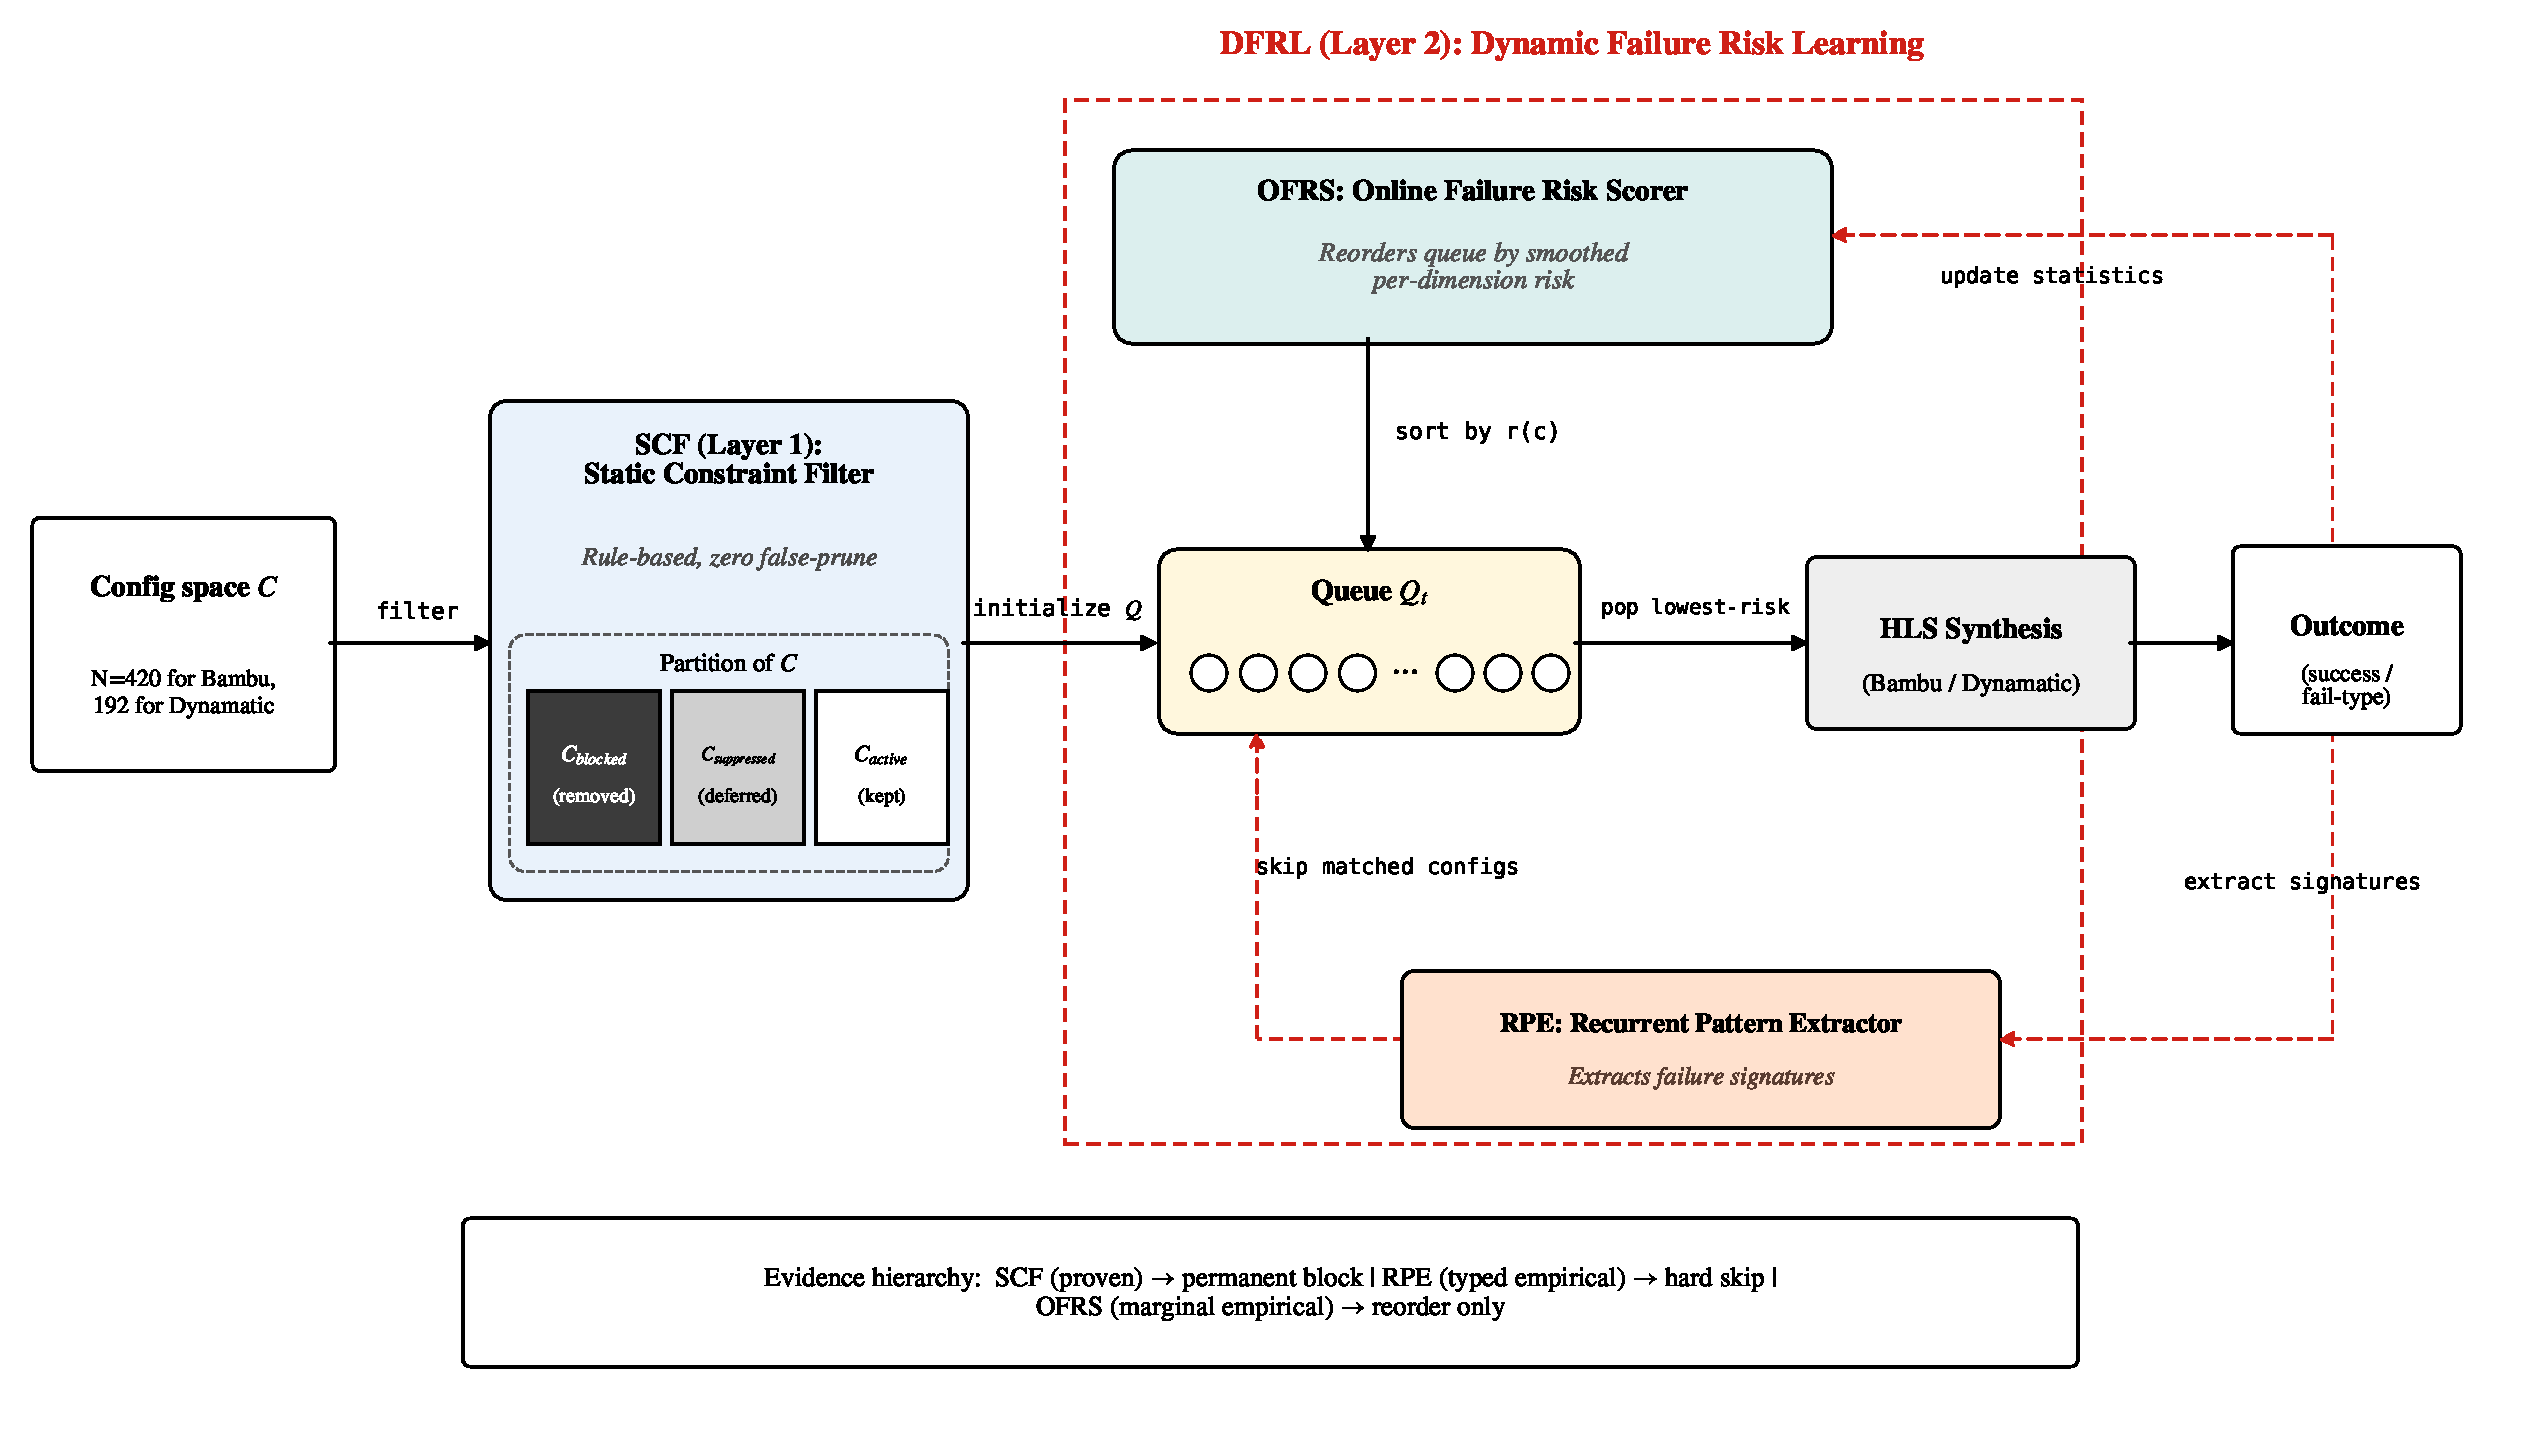
\includegraphics[width=\textwidth]{paper_figures/out/fig_architecture}
\caption{PA-DSE architecture. Layer~1 (SCF) performs offline rule-based filtering and partitions the config space $\mathcal{C}$ into \emph{blocked}, \emph{suppressed}, and \emph{active} subsets. Layer~2 (DFRL) operates online: OFRS reorders the remaining queue each iteration using smoothed per-dimension failure statistics; RPE extracts typed failure signatures from observed errors and removes matching configurations from the queue for the remainder of the run. Dashed red arrows denote the online feedback loop. Each component's action class (permanent block, hard skip, reorder) is strictly bounded by its evidence strength (bottom caption).}
\label{fig:architecture}
\end{figure*}

\subsection{Problem Setting and Policy Design}
\label{sec:formulation}

We frame feasibility-aware DSE as an \emph{online budgeted exploration problem} and describe PA-DSE as a \emph{deterministic hierarchical exploration policy} for this problem. We do not claim that PA-DSE solves an optimization problem in a formal sense; rather, we use the problem framing to clarify what the policy is trying to achieve and what trade-offs it makes.

\textbf{State.} At step $t$, the observable state is $\mathcal{S}_t = (Q_t, \mathcal{H}_t, \mathcal{P}_t, \mathcal{W}_t)$, where $Q_t$ is the remaining evaluation queue, $\mathcal{H}_t = \{(c_j, y_j)\}_{j<t}$ is the observation history with $y_j \in \{\text{success}, (\text{fail}, \text{type}_j)\}$, $\mathcal{P}_t$ is the current set of active RPE signatures, and $\mathcal{W}_t$ is the current OFRS statistics.

\textbf{Actions.} For each configuration $c \in Q_t$, the policy selects one of: \textsc{Evaluate} (consume one budget unit, observe outcome), \textsc{Skip} (permanently remove from $Q_t$), or \textsc{Defer} (reorder within $Q_t$).

\textbf{Operational goals.} The policy aims to:
\begin{enumerate}
    \item Maximize the number of feasible designs discovered within a fixed budget $B$.
    \item Minimize false skips (configurations incorrectly removed that were actually feasible).
    \item Secondarily, minimize time-to-first-feasible and maximize best-QoR-under-budget.
\end{enumerate}
These are \emph{evaluation criteria} used to assess policy quality, not formal constraints enforced by the algorithm. In particular, the false skip rate is an \emph{empirical safety target}, not an online guarantee: PA-DSE does not have a mechanism that provably bounds false skips below any threshold. Instead, it relies on the evidence hierarchy (Section~\ref{sec:hierarchy}) and conservative activation rules to keep false skips low in practice.

\textbf{Policy structure.} PA-DSE implements a deterministic, hierarchical policy:
\begin{enumerate}
    \item If $c$ matches a sound blocking rule $\rightarrow$ \textsc{Skip} (pre-exploration, provably correct).
    \item If $c$ matches an active RPE signature with sufficient evidence $\rightarrow$ \textsc{Skip} (run-scoped, empirically validated).
    \item Otherwise, rank $c$ by OFRS risk score; evaluate lowest-risk first (\textsc{Defer} high-risk configs to end of queue).
\end{enumerate}

\subsection{Evidence Hierarchy}
\label{sec:hierarchy}

PA-DSE is organized around a single design principle: \emph{action strength must not exceed evidence strength}. Table~\ref{tab:hierarchy} summarizes the mapping. Only proven constraints (tool documentation) trigger permanent, cross-run blocking. RPE signatures trigger run-scoped hard skip based on empirical evidence accumulated during exploration. OFRS influences evaluation order but never permanently excludes any configuration.

\begin{table}[t]
\centering
\caption{PA-DSE Evidence Hierarchy}
\label{tab:hierarchy}
\resizebox{\columnwidth}{!}{
\begin{tabular}{llll}
\toprule
\textbf{Evidence Source} & \textbf{Strength} & \textbf{Action} & \textbf{Scope} \\
\midrule
Tool-documented constraint   & Proven              & Permanent block     & All runs \\
Source-code heuristic        & Medium (empirical)  & Queue ordering prior & All runs \\
Recurrent failure signature  & High (empirical)    & Hard skip           & Current run \\
Per-dimension failure stats  & Low--medium         & Queue reordering    & Current run \\
\bottomrule
\end{tabular}
}
\end{table}

\subsection{Failure Taxonomy (Modeling Assumption)}
\label{sec:taxonomy}

\textbf{Assumption.} DFRL assumes that synthesis failures can be meaningfully partitioned into a small set of \emph{normalized failure categories} (error types), and that configurations sharing the same error type share exploitable structural commonalities. If this assumption is violated (for example, if distinct failure mechanisms produce the same error type, or if a single mechanism produces inconsistent error types across runs), then RPE's per-type signature extraction will degrade. The validity of this assumption is empirical and tool-dependent.

\textbf{Construction.} We define a deterministic keyword-based mapping from raw tool log output to canonical error types. For Bambu: \texttt{pipeline\_phi\_conflict}, \texttt{generic\_error}, \texttt{param\_incompatibility}. For Dynamatic: \texttt{timeout}, \texttt{buffer\_placement\_failed}. The mapping is tool-specific but deterministic: the same log output always produces the same type.

\textbf{Known limitations.} Under-splitting (different root causes $\rightarrow$ same type) dilutes RPE's ability to find consistent dimensions. Over-splitting (one root cause $\rightarrow$ multiple types) fragments the failure evidence. For example, on Dynamatic the \texttt{gemm} benchmark produces both \texttt{timeout} and \texttt{buffer\_placement\_failed} errors, limiting RPE's ability to form a single discriminative signature.

\textbf{Stability verification.} We verify cross-run consistency on a subset of 20~configurations per benchmark (same config $\rightarrow$ same error type across repeated runs) and manually spot-check 10~logs per type. The primary safeguard is the mapping's deterministic construction: identical log output always yields the same type, so instability can only arise from non-deterministic tool behavior, which we did not observe in our spot checks. A more exhaustive verification campaign covering the full configuration space would strengthen this assumption but is beyond the scope of the current work.

\subsection{Layer~1: Static Constraint Filtering (SCF)}
\label{sec:scf}

SCF partitions $\mathcal{C} = \mathcal{C}_{\text{blk}} \cup \mathcal{C}_{\text{sup}} \cup \mathcal{C}_{\text{act}}$ using a small set of hand-crafted rules, each labeled with a \emph{severity} that determines the resulting action.

\textbf{Sound blocking} ($\mathcal{C}_{\text{blk}}$): Permanently removed based on tool documentation (Bambu R1--R2). Provably correct; zero false-positive rate. Within the evidence hierarchy, this is the strongest action, reserved for proven constraints.

\textbf{Heuristic suppression} ($\mathcal{C}_{\text{sup}}$): Provides an \emph{initial queue ordering prior}: suppressed configurations are placed after active ones in the initial queue. This is not a hard exclusion: if OFRS later assigns a suppressed configuration a lower risk score than some active configurations, the suppressed configuration may be promoted ahead of them. Suppression establishes a starting bias that can be overridden by online evidence. If budget permits, all suppressed configurations are eventually evaluated.

\subsection{Layer~2: Dynamic Failure Risk Learning (DFRL)}
\label{sec:dfrl}

DFRL operates online during exploration, updating its internal state after each synthesis evaluation. It is not a classifier, surrogate model, or machine-learning method: no offline training, no gradient updates, no model fitting. Its state is fully deterministic given $\mathcal{H}_t$ and inspectable at any point.

DFRL requires the failure taxonomy assumption (Section~\ref{sec:taxonomy}) to hold for RPE, and sufficient observation volume for OFRS.

\subsubsection{Recurrent Pattern Extractor (RPE)}
\label{sec:rpe}

\textbf{Semantic scope.} RPE outputs are \emph{typed recurrent failure signatures}: parameter conditions that consistently co-occur with a specific error type and discriminate failures from successes in the current observation history. They are discriminative summaries, \emph{not} root-cause identifications. Their validity depends on observation coverage and taxonomy stability.

Within the evidence hierarchy (Section~\ref{sec:hierarchy}), RPE operates at the \emph{typed recurrent evidence} level: it requires concentrated, type-specific failure observations to trigger hard skip, the second-strongest action after sound blocking. This positioning reflects RPE's reliance on structured, repeated evidence rather than marginal or mixed-type statistics.

\textbf{Signature definition.} A signature is a tuple $\pi = (t, \mathbf{cond})$ where $t$ is a normalized error type and $\mathbf{cond} = \{(d_1, v_1), \ldots, (d_k, v_k)\}$ is a set of dimension-value pairs. A configuration $c$ \emph{matches} $\pi$, written $c \models \pi$, if and only if $c[d_i] = v_i$ for all $(d_i, v_i) \in \mathbf{cond}$.

The signature's evidence counts are defined over the \emph{entire} current observation history $\mathcal{H}_t$:
\begin{align}
n_{\text{fail}}(\pi) &= |\{(c,y) \in \mathcal{H}_t : y = (\text{fail}, t) \text{ and } c \models \pi\}| \label{eq:nfail} \\
n_{\text{counter}}(\pi) &= |\{(c,y) \in \mathcal{H}_t : y = \text{success} \text{ and } c \models \pi\}| \label{eq:ncounter}
\end{align}
That is, $n_{\text{fail}}$ counts all observed type-$t$ failures matching $\pi$, and $n_{\text{counter}}$ counts all observed successes matching $\pi$, regardless of when they were observed.

\textbf{Activation boundary.} RPE attempts signature extraction only when: (1)~$\geq \tau$ failures of the same error type $t$ exist in $\mathcal{H}_t$, and (2)~$\geq 1$ successful evaluation exists in $\mathcal{H}_t$ (providing contrast for discriminative filtering).

\textbf{Signature formation.} RPE attempts to identify, for each error type, a compact, non-redundant set of parameter conditions that captures the recurrent structure of same-type failures while excluding coincidentally shared but non-informative dimensions. The formation procedure operates as follows:

\textbf{Discriminative dimension filtering.} Given the set of all type-$t$ failures in $\mathcal{H}_t$:
\begin{enumerate}
    \item \textbf{Consistency:} For each dimension $d$, check whether all type-$t$ failures share the same value $v$. Retain only dimensions where this holds.
    \item \textbf{Discrimination:} Among retained dimensions, exclude any where $d = v$ also holds for \emph{every} observation in $\mathcal{H}_t$ (both failures and successes). Such dimensions carry no discriminative information.
    \item \textbf{Scoring:} The surviving dimensions form a candidate signature $\pi = (t, \mathbf{cond})$ with an evidence score:
\end{enumerate}
\begin{equation}
\text{conf}(\pi) = \frac{n_{\text{fail}}(\pi)}{n_{\text{fail}}(\pi) + n_{\text{counter}}(\pi) + 2}
\label{eq:confidence}
\end{equation}
The additive $+2$ in the denominator (without a matching $+1$ in the numerator) implements a conservative prior: with no observations, $\text{conf}(\pi){=}0$, so genuine failure evidence is required to raise the score. This is intentionally stronger than the symmetric add-one (Laplace) smoothing used by OFRS in Eq.~\ref{eq:ofrs_f} below, reflecting that RPE's action class (hard skip) is stronger than OFRS's (reorder). This score is a \emph{smoothed empirical evidence score}, not a calibrated probability, not a formal posterior estimate, and not a guaranteed risk bound. It summarizes the concentration of same-type failure evidence relative to counterevidence, and serves as a conservative activation gate: monotonically increasing in $n_{\text{fail}}$, monotonically decreasing in $n_{\text{counter}}$.

\textbf{Activation threshold.} A signature is activated (triggers hard skip for matching configs) only when $\text{conf}(\pi) \geq \theta$, with $\theta = 0.8$ in our experiments. To give concrete intuition: with $\theta = 0.8$, a signature with zero counterexamples requires $n_{\text{fail}} \geq 8$ to activate ($8/(8+0+2) = 0.8$). With one counterexample, it requires $n_{\text{fail}} \geq 12$ ($12/(12+1+2) = 0.8$). This means hard skip is triggered only after substantial and consistent failure evidence. The threshold $\theta$ is a user-configurable parameter; we report a sensitivity sweep across $\theta \in \{0.7, 0.8, 0.9\}$ in Section~\ref{sec:theta_sensitivity}.

\textbf{Scope and lifecycle.} Signatures are \emph{run-scoped}: they apply only within the current exploration run, not across runs or benchmarks. Within a run, signatures follow \emph{threshold-triggered activation with persistence}: once $\text{conf}(\pi) \geq \theta$, the signature becomes active and is applied to all remaining queue members. The signature remains active as long as $\text{conf}(\pi) \geq \theta$. Since evidence counts are computed over the entire history $\mathcal{H}_t$ (Eqs.~\ref{eq:nfail}--\ref{eq:ncounter}), a signature's confidence can decrease if subsequent observations add to $n_{\text{counter}}$, either through configurations evaluated before the signature was formed, or through probe auditing (below). If $\text{conf}(\pi)$ drops below $\theta$, the signature is deactivated and no longer triggers hard skip.

The lifecycle follows three rules: (1)~\emph{activation} is threshold-triggered: a signature becomes active when $\text{conf}(\pi) \geq \theta$; (2)~\emph{persistence}: an active signature remains in effect as long as $\text{conf}(\pi) \geq \theta$; (3)~\emph{deactivation} occurs only through observed counterevidence that increases $n_{\text{counter}}$ and drives $\text{conf}(\pi)$ below $\theta$. Hard-skipped configurations do not directly generate counterevidence because they are not evaluated. The only two sources of counterevidence are: (a)~configurations evaluated before the signature was formed that happen to match it and succeeded, and (b)~probe evaluations of would-be-skipped configurations.

\textbf{Probe auditing.} To provide a self-correction path, a configuration that would be hard-skipped is instead evaluated with probability $p_{\text{probe}}$ (default 0.05). If the probe succeeds, $n_{\text{counter}}$ increases and $\text{conf}(\pi)$ decreases, potentially deactivating the signature. Note that the probe Bernoulli is re-evaluated each time the skip phase encounters a matching configuration (Algorithm~\ref{alg:padse}, lines 5--11), so a configuration retained as a probe in one iteration may be removed in a subsequent one; in practice only a small expected number of probes actually consume budget. At $B{=}60$ (Bambu) and $B{=}30$ (Dynamatic), RPE does not activate and no probes are triggered. At $B{=}120$ (Bambu), RPE activates and an average of $1.0$ probe per run is evaluated, accounting for approximately $1.5\%$ of the budget actually consumed; probe outcomes are counted identically to regular evaluations in all reported metrics.

\textbf{Subsumption.} Signature $\pi_1 = (t, \mathbf{cond}_1)$ \emph{subsumes} $\pi_2 = (t, \mathbf{cond}_2)$ if: (a)~they share the same error type $t$; (b)~$\mathbf{cond}_1 \subsetneq \mathbf{cond}_2$ ($\pi_1$ has strictly fewer conditions, all of which appear in $\mathbf{cond}_2$); and (c)~$\pi_1$ is itself \emph{activated} ($\text{conf}(\pi_1) \geq \theta$). When all three conditions hold, $\pi_2$ is deactivated and removed from $\mathcal{P}_t$, because $\pi_1$ matches a strict superset of the configurations matched by $\pi_2$ and has sufficient evidence to justify hard skip on its own. Condition~(c) is critical for conservativeness: a newly formed but insufficiently supported general candidate must not displace an already-activated narrower signature.

\subsubsection{Online Failure Risk Scorer (OFRS)}
\label{sec:ofrs}

OFRS is a \emph{deliberately simple}, first-order, small-sample risk ranking model. Its sole function is queue reordering: delaying configurations with higher estimated failure association, never permanently excluding any configuration. It is not a calibrated failure predictor, probability estimator, or classifier.

Within the evidence hierarchy (Section~\ref{sec:hierarchy}), OFRS operates at the weakest evidence level: per-dimension marginal statistics that mix across failure types. This positioning dictates that OFRS may only reorder, never permanently exclude, the weakest action available.

\textbf{Why OFRS only reorders, never skips.} Unlike RPE, which operates on concentrated, high-evidence per-type signatures, OFRS aggregates marginal single-dimension statistics across all failure types. These marginal statistics are: (1)~inherently noisy at small sample sizes; (2)~unable to capture parameter interactions that may drive failure; (3)~not type-specific, so they mix evidence from structurally different failure modes. Granting OFRS skip authority would allow noisy, marginal evidence to permanently exclude configurations, including potentially Pareto-optimal feasible ones. Restricting OFRS to reordering ensures that all configurations remain reachable if budget permits, and that the only permanent exclusion mechanism (RPE) requires type-specific, concentrated, high-evidence signatures.

\textbf{Why first-order is sufficient here.} HLS infeasibility can involve parameter interactions. A higher-order model could in principle capture these, but at budgets $B \leq 80$, most pairwise $(d_1{=}v_1, d_2{=}v_2)$ combinations have 0--2 observations, making pairwise statistics unreliable. RPE handles interaction effects implicitly through its consistency-based extraction (a signature like $\{$pipeline=True$\}$ effectively captures all interactions involving pipeline). OFRS is designed to provide marginal ranking improvement as a complement to RPE, not to model failure structure independently. In interaction-dominated scenarios where no single dimension separates failure from success, all $w_d \approx 0$ and OFRS produces near-uniform rankings, gracefully degrading to no-op.

\textbf{Formulation.} For each dimension $d$ and value $v$, the smoothed failure association score is:
\begin{equation}
\hat{f}(d, v) = \frac{n_f(d{=}v) + 1}{n_f(d{=}v) + n_s(d{=}v) + 2}
\label{eq:ofrs_f}
\end{equation}
where $n_f(d{=}v)$ and $n_s(d{=}v)$ are the number of observed failures and successes, respectively, with $c[d] = v$. We use $\hat{f}$ rather than $\hat{P}$ to emphasize that this is a smoothed empirical score, not a calibrated probability estimate.

The \emph{relevance} of dimension $d$ is the range of $\hat{f}$ across its observed values:
\begin{equation}
w_d = \max_v \hat{f}(d, v) - \min_v \hat{f}(d, v)
\label{eq:relevance}
\end{equation}
with cold-start protection: $w_d = 0$ if total observations for dimension $d$ are below $n_{\min} = 5$.

The risk score for configuration $c$ is the relevance-weighted average:
\begin{equation}
r(c) = \begin{cases} \displaystyle\frac{\sum_d w_d \cdot \hat{f}(d, c[d])}{\sum_d w_d} & \text{if } \textstyle\sum_d w_d > 0 \\[6pt] 0.5 & \text{otherwise (cold-start fallback)} \end{cases}
\label{eq:risk}
\end{equation}
When $\sum_d w_d = 0$, OFRS does not alter the queue order; configurations retain the ordering established by SCF. As observations accumulate and individual dimensions cross the $n_{\min}$ threshold, OFRS gradually transitions from this passive mode (preserving the static prior) to active global reordering. This transition is smooth: each dimension independently contributes to ranking only after it has accumulated sufficient evidence, so OFRS's influence grows incrementally rather than switching on abruptly.

\subsection{Module Interface Specification}
\label{sec:interface}

The two layers yield four distinct operations that interact through a well-defined priority ordering, each reflecting the evidence hierarchy principle that action strength must not exceed evidence strength:

\textbf{1. Sound blocking (SCF)} permanently removes configurations from the design space before exploration begins. This action is irreversible and provably correct (zero false positives). \emph{Evidence: proven constraints. Action: strongest (permanent block).}

\textbf{2. Heuristic suppression (SCF)} establishes an \emph{initial queue ordering prior}: suppressed configurations are placed after active ones. This is \emph{not} a hard exclusion; it is an ordering bias that OFRS may override as evidence accumulates. In practice, suppressed configurations typically receive high risk scores from OFRS (because they match failure-prone parameter combinations), so OFRS tends to reinforce rather than contradict the static prior. \emph{Evidence: medium (empirical). Action: ordering bias, overridable.}

\textbf{3. RPE hard skip} removes matching configurations from the queue during exploration. RPE operates independently of OFRS: it removes configs before OFRS ranks the remainder. A configuration may be simultaneously suppressed (by SCF) and RPE-skipped; the skip takes precedence. \emph{Evidence: high (empirical, typed, concentrated). Action: run-scoped permanent removal.}

\textbf{4. OFRS reordering} sorts the remaining queue by risk score. This is a global sort over all remaining configurations, both active and suppressed. OFRS reordering is the weakest action: it never removes configurations, only changes their evaluation order. \emph{Evidence: low--medium (marginal, mixed-type). Action: weakest (reorder only).}

\textbf{Conflict handling.} OFRS may promote a heuristically-suppressed configuration ahead of active ones if its risk score is lower. This is by design: OFRS reacts to actual synthesis evidence, which may reveal that a suppressed configuration's non-suppression parameters are associated with success. Since OFRS only promotes (evaluates earlier, not skips), the worst case is one wasted budget unit, which is always preferable to permanently excluding a potentially feasible design.

\textbf{Cold-start window.} During the first $\sim n_{\min}$ evaluations, OFRS has insufficient data for meaningful relevance scores. During this period, queue order follows the SCF prior (active before suppressed). RPE also requires $\geq \tau$ same-type failures before activating, so early exploration proceeds without dynamic intervention.

\subsection{Exploration Algorithm}

Algorithm~\ref{alg:padse} summarizes the PA-DSE policy. Newly learned RPE signatures take effect in the next iteration of the while loop, not retroactively.

\begin{algorithm}[!htbp]
\caption{PA-DSE Exploration Policy}
\label{alg:padse}
\begin{algorithmic}[1]
\REQUIRE $\mathcal{C}$, source $S$, budget $B$, threshold $\tau$, probe rate $p_{\text{probe}}$
\ENSURE Results $\mathcal{R}$
\STATE $\mathcal{C}_{\text{act}}, \mathcal{C}_{\text{blk}}, \mathcal{C}_{\text{sup}} \leftarrow \text{SCF}(\mathcal{C}, S)$
\STATE $Q \leftarrow \mathcal{C}_{\text{act}} \mathbin\Vert \mathcal{C}_{\text{sup}}$; $n \leftarrow 0$
\WHILE{$Q \neq \emptyset$ \AND $n < B$}
    \FOR{$c \in Q$}
        \IF{RPE.matches($c$)}
            \IF{rand() $< p_{\text{probe}}$}
                \STATE mark $c$ as probe
            \ELSE
                \STATE remove $c$ from $Q$ \COMMENT{Hard skip}
            \ENDIF
        \ENDIF
    \ENDFOR
    \STATE Sort $Q$ by $r(c)$ ascending \COMMENT{OFRS: global reorder}
    \STATE $c \leftarrow Q.\text{popFirst}()$; $n \leftarrow n + 1$
    \STATE $(\text{ok}, \text{met}, \text{out}) \leftarrow \text{Synthesize}(c, S)$
    \IF{ok}
        \STATE OFRS.update($c$, success)
        \IF{$c$ is probe}
            \STATE RPE.addCounter($c$)
        \ENDIF
    \ELSE
        \STATE OFRS.update($c$, failure)
        \STATE RPE.tryExtract(out, $c$, $\tau$)
    \ENDIF
    \STATE $\mathcal{R} \leftarrow \mathcal{R} \cup \{(c, \text{met}, \text{ok})\}$
\ENDWHILE
\RETURN $\mathcal{R}$
\end{algorithmic}
\end{algorithm}


\section{Experimental Setup}
\label{sec:setup}

\subsection{Tools and Benchmarks}

We evaluate PA-DSE on two HLS tools that differ fundamentally in scheduling philosophy:
\begin{itemize}
    \item \textbf{PandA-Bambu v0.9.8}~\cite{pilato2013bambu}: statically scheduled, C-centric, with a well-established failure-taxonomy surface.
    \item \textbf{Dynamatic v2.0}~\cite{josipovic2018dynamically}: dynamically scheduled (elastic dataflow), LLVM-based, with MILP-driven buffer placement (solved using Gurobi 12.0 in our setup).
\end{itemize}
This pairing stresses tool-generality: the two tools share no pragma vocabulary, expose disjoint failure modes, and benefit asymmetrically from static versus dynamic pruning, as we analyze below.

\textbf{Benchmarks.} Both tools are evaluated on the same eight benchmarks: \texttt{matmul}, \texttt{vadd}, \texttt{fir}, \texttt{histogram}, \texttt{atax}, \texttt{bicg}, \texttt{gemm}, and \texttt{gesummv}. The selection combines Polybench linear-algebra kernels and simple DSP kernels, covering a range of loop-nest structures and feasibility landscapes. We chose benchmarks that are present in both tools' integration-test suites to enable cross-tool comparison; CHStone and MachSuite benchmarks were considered but require non-trivial porting to Dynamatic's LLVM-based frontend. Using the same benchmark set on both tools enables direct cross-tool comparison of failure-mode structure and PA-DSE behavior. (Dynamatic's integration-test suite names the matrix-multiplication kernel \texttt{matrix}; we use \texttt{matmul} throughout for consistency.)

\subsection{Configuration Spaces}

\textbf{Bambu (420 configurations).} The enumerated space is the Cartesian product of memory controller choices (\texttt{channels\_type} $\in$ \{\texttt{MEM\_ACC\_11}, \texttt{MEM\_ACC\_N1}, \texttt{MEM\_ACC\_NN}\}), channel count (\texttt{channels\_number} $\in \{1, 2, 4\}$), target clock period, loop pipelining on/off, and further binding/scheduling options. Two tool-documented incompatibilities contribute a provably infeasible \emph{blocked} subset $\mathcal{C}_{\text{blk}}$ of size $140$ ($33.3\%$): MEM\_ACC\_11 requires exactly one channel, MEM\_ACC\_NN requires at least two. In addition, source-level heuristics (pipelining interacting with accumulation or control-flow patterns) mark up to $224$ configurations as \emph{suppressed} for a subset of benchmarks (\texttt{matmul}, \texttt{fir}, \texttt{histogram}); these are deferred but not removed from the queue.

\textbf{Dynamatic (192 configurations).} The enumerated space covers target clock period, buffer algorithm (\texttt{on\_merges}, \texttt{fpga20}, \texttt{fpl22}), hardware sharing, LSQ sizing, and fast-token-delivery tuning. \emph{No tool-documented incompatibility rules apply to this space,} so under SCF all 192 configurations remain in the active set: $\mathcal{C}_{\text{blk}} = \emptyset$ and $\mathcal{C}_{\text{sup}} = \emptyset$. SCF-on and SCF-off behave identically on Dynamatic, making this tool a deliberate stress test of whether DFRL can carry the feasibility-aware load on its own (Section~\ref{sec:ablation}).

\textbf{Feasibility landscape asymmetry.} Three of the eight benchmarks (\texttt{vadd}, \texttt{fir}, and \texttt{histogram}) achieve $100\%$ ground-truth feasibility on Dynamatic: all 192 configurations synthesize successfully regardless of buffer algorithm, clock period, or sharing options. This contrasts with Bambu, where the same three benchmarks exhibit the same $\sim\!15\%$ random-sampling SR as all other benchmarks, because Bambu's dominant infeasibility source (MEM\_ACC parameter incompatibilities) is source-independent.

The difference reflects a structural asymmetry in failure mechanisms. On Bambu, infeasibility is \emph{pragma-driven}: tool-level parameter rules (R1--R2) reject configurations regardless of source complexity. On Dynamatic, infeasibility is \emph{graph-complexity-driven}: the MILP-based buffer-placement solver's difficulty scales with the dataflow graph's back-edge count and path interactions, so simple kernels with flat loop structures are trivially solvable while complex kernels (\texttt{gemm}, ground-truth SR $35.4\%$; \texttt{matmul}, $45.8\%$) produce substantial failure fractions. This asymmetry validates the two-layer design: SCF addresses pragma-driven failures (Bambu), while DFRL addresses graph-complexity-driven failures (Dynamatic). Because the three trivially feasible benchmarks carry no discriminative signal (all methods achieve $100\%$ SR), we report aggregate Dynamatic metrics over the five non-trivial benchmarks (\texttt{matmul}, \texttt{atax}, \texttt{bicg}, \texttt{gemm}, \texttt{gesummv}). Per-benchmark results for all eight benchmarks are shown in Figure~\ref{fig:heatmap} for completeness.

\subsection{Baselines}
\label{sec:baselines}

We compare against six baselines chosen to span the classical and learned HLS DSE landscape:

\begin{itemize}
    \item \textbf{Random}: uniform sampling without replacement from $\mathcal{C}$.
    \item \textbf{Filtered Random}: uniform sampling from $\mathcal{C} \setminus \mathcal{C}_{\text{blk}}$, i.e.\ a strict SCF-only baseline. On Dynamatic this reduces to Random since $\mathcal{C}_{\text{blk}} = \emptyset$.
    \item \textbf{Simulated Annealing (SA)} and \textbf{Genetic Algorithm (GA)}: classical black-box optimizers using feasibility as fitness~\cite{ferretti2020cluster,liu2013learning}.
    \item \textbf{Bayesian Optimization (GP-BO)}: Gaussian-process surrogate with expected-improvement acquisition, following the BO-for-HLS-DSE line of work~\cite{snoek2012practical,ferretti2018lattice}.
    \item \textbf{Random Forest Classifier (RF)}: an online-trained binary feasibility classifier ($n_{\text{estimators}}{=}100$, retrained from scratch after every synthesis call using all observations collected so far). At each step, RF predicts feasibility for all remaining configurations; those with predicted probability $\geq 0.6$ are sampled uniformly. If no configuration exceeds the threshold, one is drawn at random. This is a simplified online proxy inspired by the scalable surrogate of AutoScaleDSE~\cite{sohrabizadeh2023autoscaledse}; it differs from the original in that it trains online within a single run rather than on an offline corpus across designs.
\end{itemize}

All baselines share the same $\mathcal{C}$, the same synthesis interface, and the same per-run budget.

\subsection{Evaluation Protocol}
\label{sec:protocol}

\textbf{Budgets.} We use $B{=}60$ evaluations per run on Bambu and $B{=}30$ on Dynamatic. These are chosen to represent realistic ``coffee-break'' interactive budgets: with per-call synthesis cost of $\approx 2.5$\,s (Bambu) and $\approx 8$\,s (Dynamatic), a full run completes in 2--4 minutes of wall clock in both cases. We also sweep $B \in \{30, 60\}$ in the Bambu ablation.

\textbf{Repetitions.} Each (method, benchmark, budget) cell is repeated 10 times. For stochastic baselines (Random, SA, GA, GP-BO, RF) the repetition index is a random seed. For deterministic methods (Filtered Random, PA-DSE) we vary the initial queue ordering via a \texttt{queue\_permutation\_id}, which is mechanically equivalent to a seed for sensitivity analysis. This isolates ordering sensitivity from optimizer-internal randomness.

\textbf{PA-DSE hyperparameters.} We freeze $\tau{=}2$ (minimum failure support for RPE signature activation), $\theta{=}0.8$ (RPE confidence threshold), $n_{\min}{=}5$ (OFRS cold-start observation threshold), and $p_{\text{probe}}{=}0.05$ (probe rate for keeping active signatures honest). These defaults are not tuned per-benchmark or per-tool.

\textbf{Metrics.} We report:
\begin{itemize}
    \item \textbf{SR (\%)}: fraction of evaluated configurations that synthesized successfully, the primary feasibility metric.
    \item \textbf{Wasted calls}: count of synthesis invocations that returned a failure, a proxy for user-visible time cost.
    \item \textbf{TTFF (s)}: wall-clock time to first feasible design, relevant for interactive use.
    \item \textbf{UQoR}: number of unique Pareto-eligible QoR points (distinct (area, latency) pairs) discovered.
    \item \textbf{Best area, best latency}: minima observed across successful configurations in the run.
    \item \textbf{Algorithmic overhead}: per-iteration time spent in each PA-DSE layer (\texttt{overhead\_scf\_ms}, \texttt{overhead\_rpe\_ms}, \texttt{overhead\_ofrs\_ms}).
\end{itemize}

\textbf{Hardware.} All runs execute single-threaded on an Azure \texttt{Standard\_D4s\_v5} VM (4 vCPUs, 15\,GB RAM, Ubuntu 24.04, Python 3.12). No GPUs are used. Gurobi 12.0 (academic license) is used for Dynamatic's MILP buffer placement.

\textbf{Reproducibility.} Code, configuration generators, benchmark sources, raw run logs, and all aggregation scripts are released at \url{https://github.com/jane09250410/hls-dse}. A single \texttt{run\_all.sh} regenerates every table and figure in this paper.


\section{Results}
\label{sec:results}

We structure the evaluation around nine questions, each addressed in its own subsection:
(1)~Does PA-DSE outperform classical and learned baselines on success rate?
(2)~How large is the user-visible cost savings in terms of wasted calls and TTFF?
(3)~Are per-benchmark results consistent, or driven by a few easy benchmarks?
(4)~What does the convergence trajectory look like? Does PA-DSE reach its SR early or late in the budget?
(5)~Does PA-DSE's queue reordering sacrifice QoR quality?
(6)~Does the ablation confirm the evidence-hierarchy design principle?
(7)~How sensitive is PA-DSE to the RPE confidence threshold $\theta$?
(8)~Does RPE contribute at extended budgets where it activates?
(9)~Is the algorithmic overhead of PA-DSE negligible relative to synthesis cost?

% ------------------------------------------------------------
\subsection{Main Comparison on Bambu}
\label{sec:main_results}

Table~\ref{tab:main_bambu} reports per-method means and standard deviations across all $(benchmark, \text{run})$ cells on Bambu at $B{=}60$. PA-DSE achieves $92.5\% \pm 1.1$ success rate, exceeding the strongest baseline (RF, $85.9\% \pm 1.1$) by $6.6$\,pp. More importantly, PA-DSE wastes only $4.5$ synthesis calls on average per run, compared to $8.4$ for RF, $17.2$ for GP-BO, and $51.0$ for Random, a $\mathbf{1.9\times}$ reduction over the best baseline and an $\mathbf{11\times}$ reduction over Random. Because each wasted call costs $\approx 2.5$\,s of user time on Bambu, PA-DSE saves roughly $10$\,s of wall clock per run versus RF.

\begin{table*}[t]
\centering
\caption{Main results on Bambu ($B{=}60$, $n{=}80$ runs per method: 8 benchmarks $\times$ 10 seeds/permutations). PA-DSE's $\sigma$ reflects queue-permutation variation; other methods' $\sigma$ reflects seed variation.}
\label{tab:main_bambu}
\resizebox{\textwidth}{!}{
\begin{tabular}{lrrrrrr}
\toprule
Method & SR (\%) & Wasted & TTFF (s) & UQoR & Best area & Best latency \\
\midrule
Random         & 15.0 \std{2.5}  & 51.0 & 22.9 &  6.4 & 473.1 & 10.94 \\
Filtered Random& 18.5 \std{3.4}  & 48.9 & 11.9 &  7.9 & 473.9 & 10.94 \\
SA             & 18.4 \std{29.4} & 49.0 &  2.5 &  4.3 & 464.1 & 10.58 \\
GA             & 50.6 \std{26.8} & 29.6 &  7.7 & 11.8 & 464.1 & 10.61 \\
GP-BO          & 71.3 \std{7.0}  & 17.2 & 10.9 & 14.9 & 464.1 & 10.28 \\
RF             & 85.9 \std{1.1}  &  8.4 & 14.3 & 17.1 & 464.1 & 10.31 \\
\textbf{PA-DSE}& \textbf{92.5} \std{1.1} & \textbf{4.5} & 8.9 & \textbf{19.1} & \textbf{464.1} & \textbf{10.25} \\
\bottomrule
\end{tabular}
}
\end{table*}

Two additional observations are worth noting. First, PA-DSE shows minimal sensitivity to initial queue permutation, with $\sigma{=}1.1$ across 10 permutations on Bambu. RF reports $\sigma{=}1.1$ across 10 seeds; the two $\sigma$ values measure different sources of variation (permutation-induced ordering vs.\ optimizer-internal randomness) and should not be compared directly as a robustness claim. Simulated annealing, by contrast, has $\sigma{=}29.4$: some runs find feasible configurations early and succeed, while others get trapped in infeasible regions; this reflects a broader pattern that classical black-box methods are ill-suited to design spaces dominated by structural infeasibility. Second, on Bambu PA-DSE matches the best area of every baseline ($464.1$, tied at the tool's lower bound), achieves the lowest best latency among all methods ($10.25$ cycles), and the highest UQoR ($19.1$); the cross-tool picture is more nuanced and is discussed in \S\ref{sec:dynamatic_results}. Figure~\ref{fig:bambu_main} visualizes the full per-method distribution.



\begin{figure}[t]
\centering
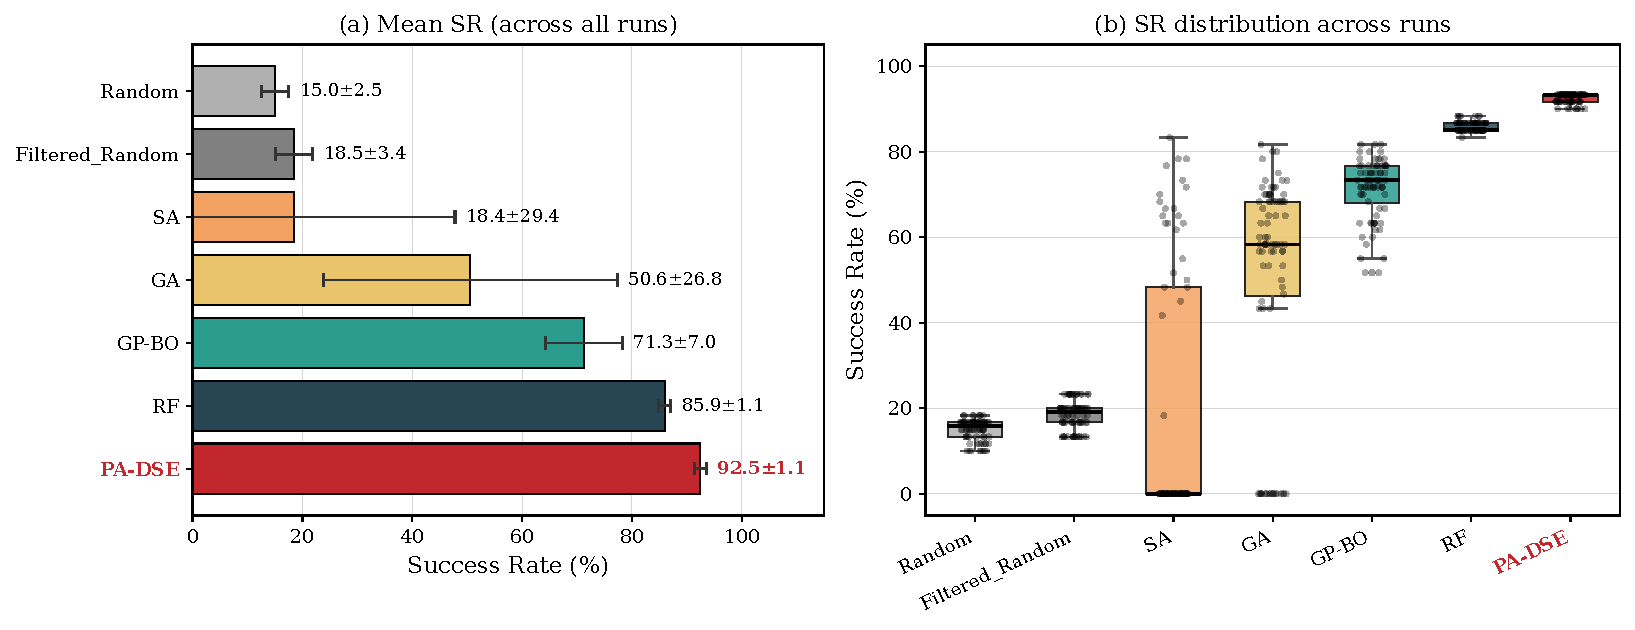
\includegraphics[width=\columnwidth]{paper_figures/out/fig1_bambu_main.pdf}
\caption{Bambu main results ($B{=}60$). (a) Mean SR with standard deviation error bars. (b) Per-run SR distribution: PA-DSE matches the tightest $\sigma$ ($1.1$) among methods with non-trivial SR, while reaching the highest mean.}
\label{fig:bambu_main}
\end{figure}

% ------------------------------------------------------------
\subsection{Cross-Tool Evaluation on Dynamatic}
\label{sec:dynamatic_results}

Table~\ref{tab:main_dynamatic} reports results on Dynamatic at $B{=}30$, aggregated over the five benchmarks with non-trivial failure rates. Because Dynamatic exposes no tool-documented incompatibility rules ($\mathcal{C}_{\text{blk}} = \emptyset$), SCF reduces to a no-op; Filtered Random is identical to Random, and the SCF-only ablation matches no-filter (Section~\ref{sec:ablation}). Any improvement over Random must therefore come from DFRL.

\begin{table*}[t]
\centering
\caption{Main results on Dynamatic ($B{=}30$, $n{=}50$ runs per method: 5 non-trivial benchmarks $\times$ 10 seeds/permutations). Filtered Random $=$ Random because $\mathcal{C}_{\text{blk}} = \emptyset$. Three benchmarks (\texttt{vadd}, \texttt{fir}, \texttt{histogram}) achieve $100\%$ SR for all methods and are excluded from aggregation.}
\label{tab:main_dynamatic}
\resizebox{\textwidth}{!}{
\begin{tabular}{lrrrrrr}
\toprule
Method & SR (\%) & Wasted & TTFF (s) & UQoR & Best area & Best latency \\
\midrule
Random         & 49.9 \std{12.8} & 15.0 & 36.6 & 9.3 & 51.7 & 404.0 \\
Filtered Random& 49.9 \std{12.8} & 15.0 & 36.6 & 9.3 & 51.7 & 404.0 \\
SA             & 49.4 \std{24.5} & 15.2 & 64.7 & 7.4 & 52.8 & 408.7 \\
GA             & 64.5 \std{13.4} & 10.6 & 36.6 & 8.5 & 51.2 & 403.7 \\
GP-BO          & 90.2 \std{4.9}  &  2.9 & 67.0 & 5.1 & 51.3 & 405.4 \\
RF             & 85.6 \std{5.8}  &  4.3 & 67.0 & 6.1 & 51.3 & 413.0 \\
\textbf{PA-DSE}& \textbf{91.3} \std{3.9} & \textbf{2.6} & \textbf{34.2} & 7.1 & 51.3 & 407.6 \\

\bottomrule
\end{tabular}
}
\end{table*}

PA-DSE achieves $91.3\%$ SR, compared to GP-BO ($90.2\%$) and RF ($85.6\%$). The more distinctive advantage over GP-BO is in user-visible cost: TTFF drops to $34.2$\,s versus $67.0$\,s for GP-BO and RF, roughly half the wall-clock time, and Wasted drops to $2.6$ versus $2.9$ and $4.3$. For interactive developers iterating tens of times a day, this compounds to significant time savings. Figure~\ref{fig:dynamatic_main} shows the per-benchmark distribution.

\textbf{Reading the QoR columns.} The last three columns (UQoR, best area, best latency) require careful reading. Among methods with SR $\geq 85\%$ (GP-BO, RF, and PA-DSE), best latency values are comparable: PA-DSE $407.6$, GP-BO $405.4$, RF $413.0$. The lat-stronger baselines (Random $404.0$, GA $403.7$) sample the design space broadly; this broad sampling occasionally discovers low-latency configurations that PA-DSE does not reach within the limited budget, but the same broad sampling is what produces their catastrophic SR ($49.9\%$, $64.5\%$) and Wasted counts ($10$--$15$). Restated: \emph{a method that wastes one third to one half of its budget on infeasible configurations does occasionally bump into a low-latency point, but is not a viable production policy}. PA-DSE's UQoR ($7.1$) leads all SR $\geq 85\%$ baselines (GP-BO $5.1$, RF $6.1$), indicating that feasibility-focused queue reordering does not sacrifice QoR diversity.



\begin{figure}[t]
\centering
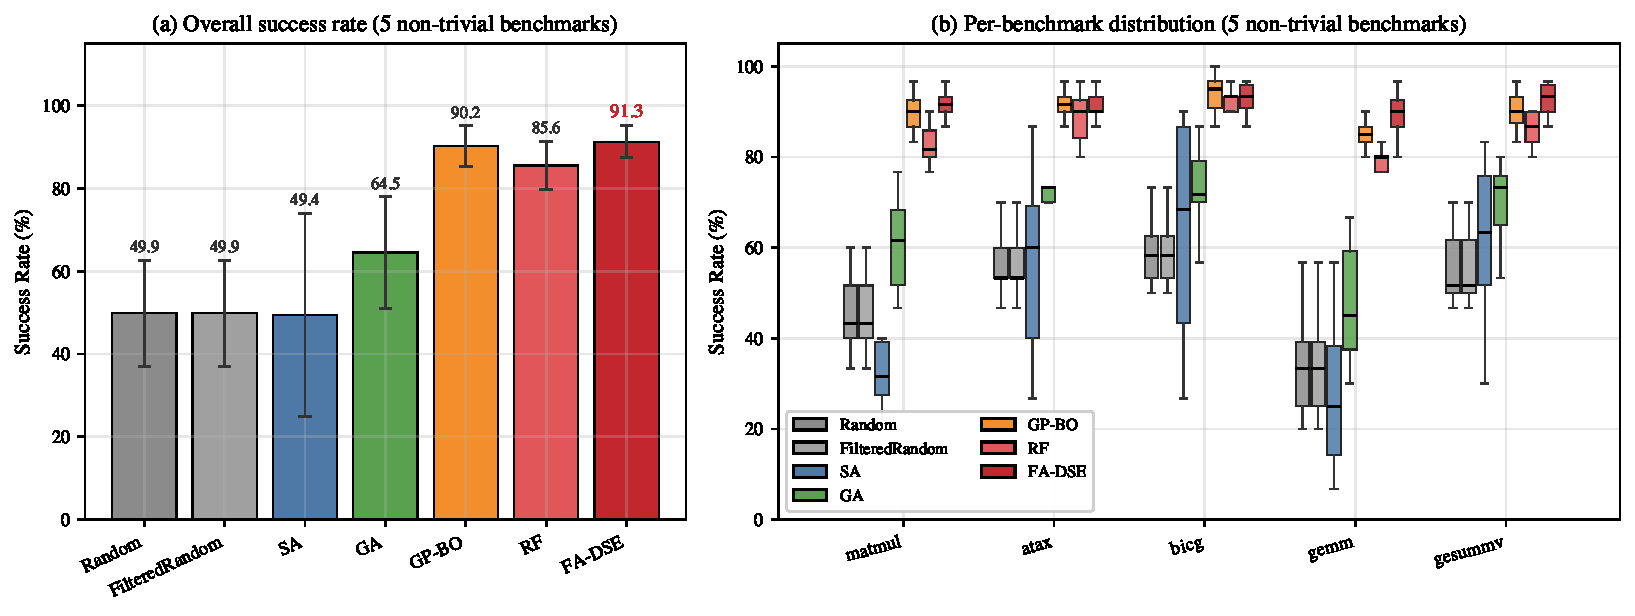
\includegraphics[width=\columnwidth]{paper_figures/out/fig_dynamatic_main.pdf}
\caption{Dynamatic main results ($B{=}30$). (a) Aggregate SR with standard deviation across five non-trivial benchmarks. (b) Per-benchmark SR distribution. PA-DSE achieves the highest aggregate SR and remains competitive across non-trivial Dynamatic benchmarks, with lower variance among deployable methods.}
\label{fig:dynamatic_main}
\end{figure}

% ------------------------------------------------------------
\subsection{User-Visible Cost: Wasted Calls and Time-to-First-Feasible}
\label{sec:cost}

Success rate is only one dimension of user experience; two others dominate perceived quality in interactive DSE: how many synthesis calls are wasted (each wasted call is a direct time cost) and how quickly the first feasible design is found (influences iteration speed). Figure~\ref{fig:cost} summarizes both.

\begin{figure*}[t]
\centering
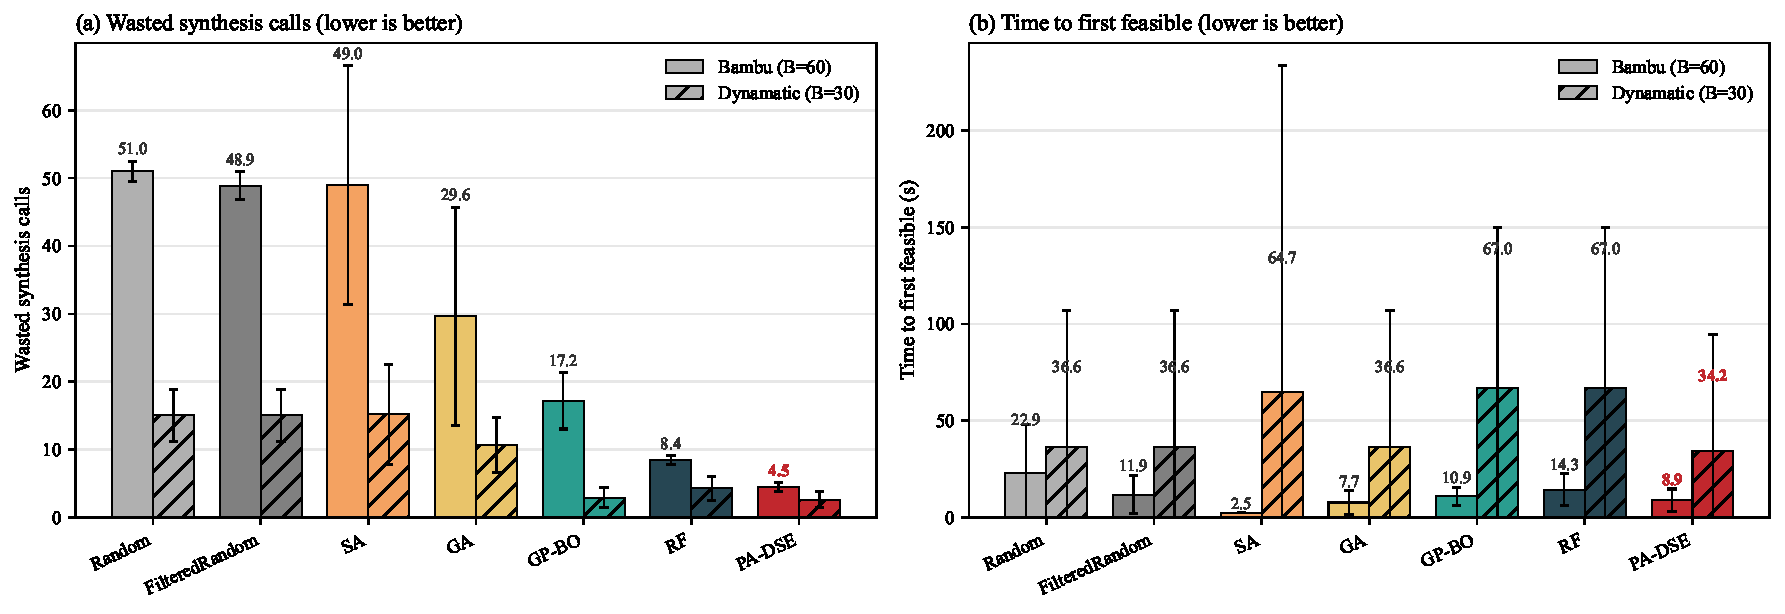
\includegraphics[width=\textwidth]{paper_figures/out/fig_cost.pdf}
\caption{User-visible cost. (a) Wasted synthesis calls per run (lower is better): PA-DSE wastes $4.5$ on Bambu ($1.9\times$ fewer than RF) and $2.6$ on Dynamatic (vs.\ $2.9$ for GP-BO and $4.3$ for RF). (b) Time to first feasible (lower is better): on Dynamatic, PA-DSE reaches the first feasible design in half the wall-clock time of GP-BO and RF.}
\label{fig:cost}
\end{figure*}

PA-DSE wastes $4.5$ synthesis calls per run on Bambu ($11.3\times$ fewer than Random, $1.9\times$ fewer than RF) and $2.6$ on Dynamatic (vs.\ $2.9$ for GP-BO and $4.3$ for RF). Translated to wall-clock: on Bambu, PA-DSE saves about $10$\,s per run versus RF ($\approx 4$ calls $\times$ 2.5\,s); on Dynamatic, about $2$\,s per run versus GP-BO ($\approx 0.3$ calls $\times$ 8.1\,s) and about $14$\,s versus RF ($\approx 1.7$ calls $\times$ 8.1\,s). For interactive developers iterating tens of times a day, this compounds to meaningful time savings. TTFF shows a similar picture on Dynamatic ($34.2$\,s for PA-DSE vs.\ $67.0$\,s for GP-BO/RF); on Bambu, classical methods have unusually low TTFF because they find occasional trivial successes early, but their mean SR is much lower (Table~\ref{tab:main_bambu}).

% ------------------------------------------------------------
\subsection{Per-Benchmark Consistency}
\label{sec:perbench}

Aggregate SR can mask method-benchmark interactions: a method might win on average while failing badly on a specific benchmark. Figure~\ref{fig:heatmap} plots mean SR for every (method, benchmark) cell.

\begin{figure*}[t]
\centering
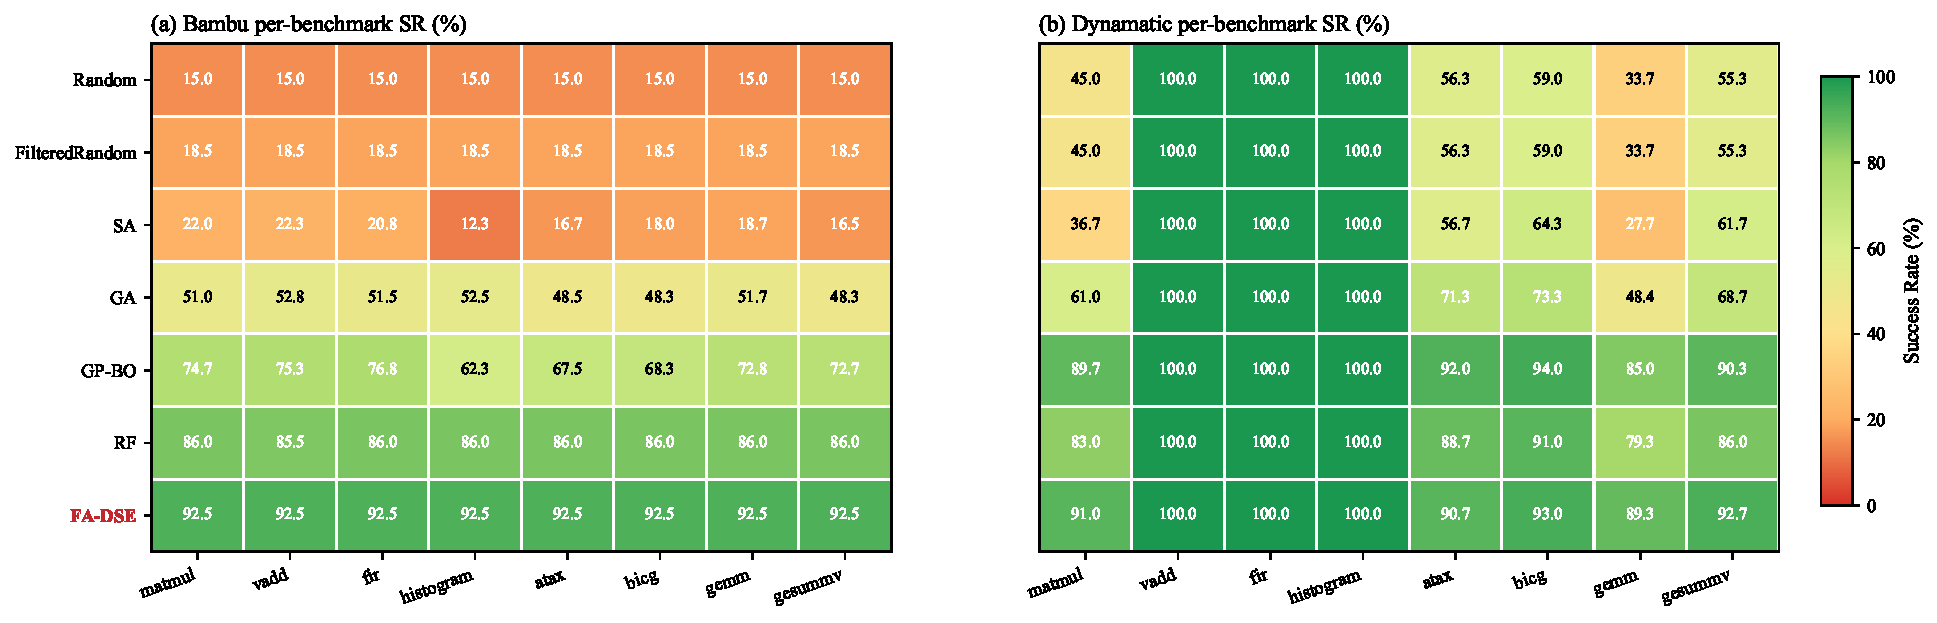
\includegraphics[width=\textwidth]{paper_figures/out/fig_perbench_heatmap.pdf}
\caption{Per-benchmark success rate (\%). PA-DSE is consistently high across benchmarks: it wins or ties on all Bambu benchmarks and remains competitive on all Dynamatic benchmarks, with low per-run variance. Several rows in panel~(a) appear flat; this is structural, not an artifact (\S\ref{sec:perbench}).}
\label{fig:heatmap}
\end{figure*}

PA-DSE achieves $\geq 90\%$ SR on every Bambu benchmark, while every baseline (including RF) has at least one benchmark where it drops noticeably. SA and GA in particular show high per-benchmark variance, consistent with their sensitivity to the benchmark-specific feasibility landscape. On Dynamatic, per-benchmark variation is more pronounced than on Bambu, reflecting the graph-complexity-driven nature of Dynamatic's failure modes. Three benchmarks (\texttt{vadd}, \texttt{fir}, \texttt{histogram}) achieve $100\%$ SR for all methods due to their trivially simple dataflow graphs. Among the five non-trivial benchmarks, \texttt{gemm} is the hardest (ground-truth feasibility $35.4\%$), and PA-DSE achieves $89.3\%$ SR, outperforming GP-BO and RF by the widest margins in the evaluation. This pattern (PA-DSE's advantage growing on harder benchmarks) is consistent with OFRS learning the dominant failure dimension (\texttt{buffer\_algorithm}: \texttt{on-merges} achieves $0\%$ failure rate, while \texttt{fpl22} reaches $82.5\%$) early and concentrating budget on feasible configurations.

\paragraph{Why some Bambu rows are nearly benchmark-agnostic.} Several rows in Figure~\ref{fig:heatmap}(a) (Random, Filtered Random, RF, and PA-DSE) show essentially identical SR across all eight benchmarks. This is structural, not an artifact, and results from three properties acting together: (1)~the dominant infeasibility band ($\mathcal{C}_{\text{blk}}$, $33\%$ of $\mathcal{C}$) is determined by tool-level MEM\_ACC rules that are independent of source code; (2)~memoryless methods derive their evaluation order from a fixed seed or permutation ID without consulting source features, so the same 60-config sequence is examined on every benchmark; and (3)~at $B{=}60$, the active set $\mathcal{C}_{\text{act}}$ alone exceeds the budget on every benchmark, so suppressed configurations are never reached, and benchmarks with and without $\mathcal{C}_{\text{sup}}$ behave identically. By contrast, GP-BO, SA, and GA carry benchmark-specific internal state that produces genuine per-benchmark variation. On Dynamatic, failure modes are source-dependent, so PA-DSE's per-benchmark SR varies across benchmarks depending on graph complexity.

% ------------------------------------------------------------
\subsection{Convergence Behavior}
\label{sec:convergence}

Figure~\ref{fig:convergence} shows the cumulative number of feasible designs found as a function of the evaluation step, averaged across runs. This reveals not just the \emph{amount} of budget used but the \emph{trajectory}: does PA-DSE front-load its successes or find them throughout?

\begin{figure*}[t]
\centering
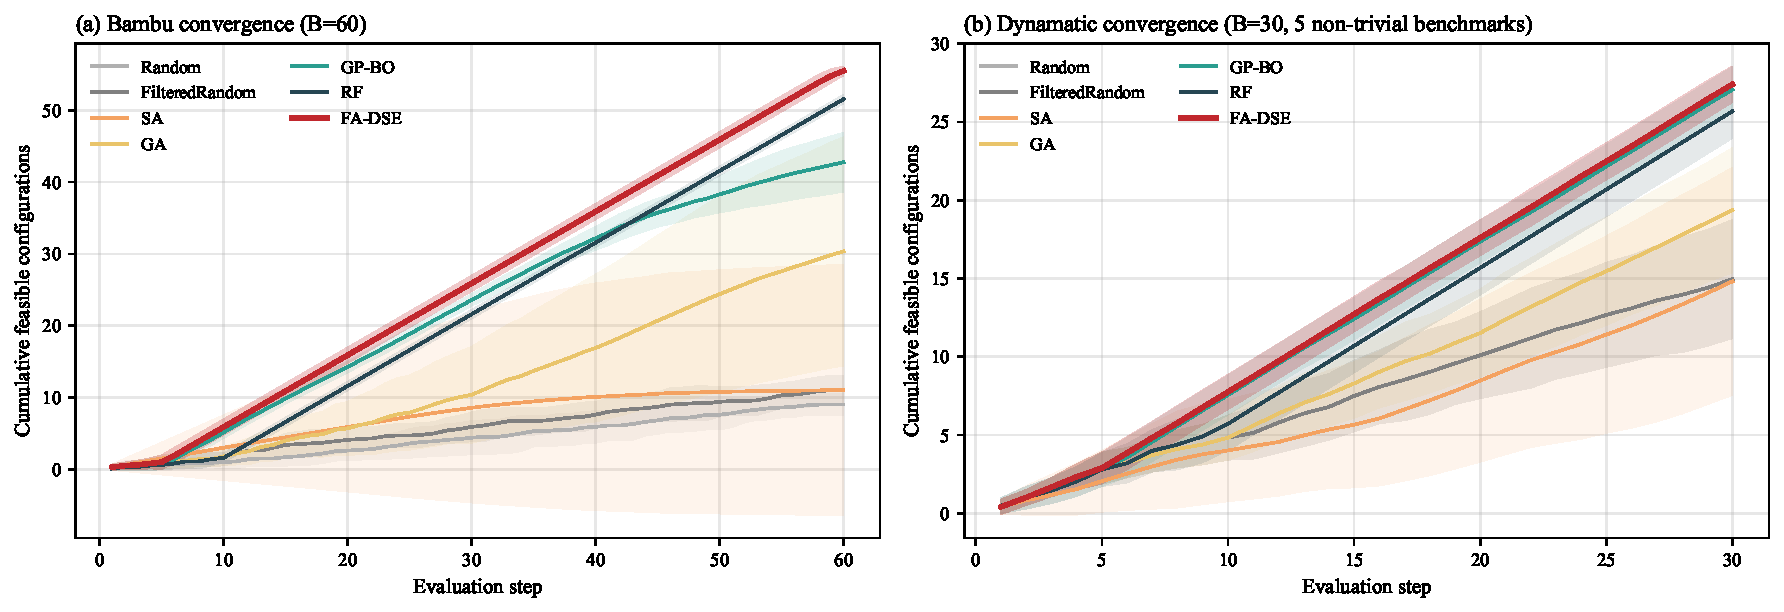
\includegraphics[width=\textwidth]{paper_figures/out/fig_convergence.pdf}
\caption{Convergence curves (mean $\pm 1\sigma$ across runs). (a) Bambu at $B{=}60$: PA-DSE maintains near-linear progression throughout the budget, indicating that OFRS's online reordering keeps promising configurations at the queue front. (b) Dynamatic at $B{=}30$: PA-DSE's curve is steeper than the classical baselines, reflecting rapid learning of the dominant failure dimension.}
\label{fig:convergence}
\end{figure*}

On Bambu (panel a), PA-DSE's curve rises nearly linearly through the full 60-step budget, reflecting that DFRL continually surfaces feasible configurations rather than finding them all early and then stalling. RF catches up toward the tail; SA and GA exhibit characteristic stagnation. On Dynamatic (panel b), PA-DSE converges within the first $\sim 20$ steps to $\approx 28$ feasibles, while classical methods ($<20$ feasibles at step $30$) never catch up.

% ------------------------------------------------------------
\subsection{Quality of Results (QoR)}
\label{sec:qor}

Finding feasible configurations is necessary but not sufficient; users ultimately want coverage of the (area, latency) quality space, especially near the Pareto front. We evaluate QoR coverage by overlaying the unique (area, latency) points discovered by PA-DSE and the union of all baselines. Each tool's plot in Figure~\ref{fig:qor} categorizes every unique QoR point by which method(s) found it: \emph{shared} (both PA-DSE and at least one baseline), \emph{baseline-only} (no PA-DSE run found it), and Pareto-front markers (large diamonds). The annotation in each panel reports PA-DSE's coverage of the Pareto-optimal vertices.

\begin{figure*}[t]
\centering
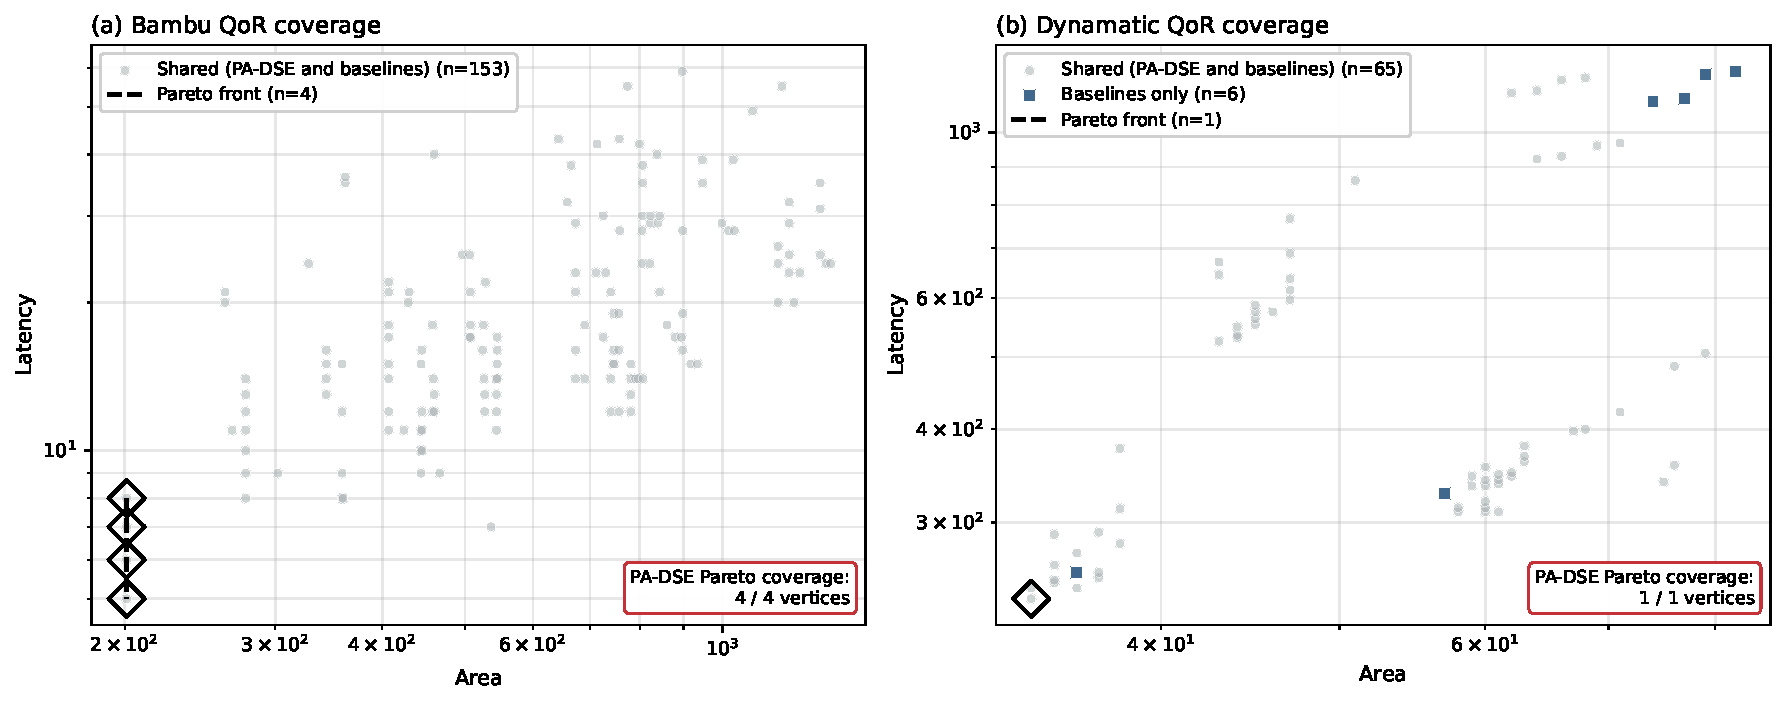
\includegraphics[width=\textwidth]{paper_figures/out/fig_qor.pdf}
\caption{QoR coverage comparison: each panel overlays the unique (area, latency) points discovered by PA-DSE and the union of baselines. \emph{Shared} points (gray) are found by both; \emph{baseline-only} points (blue) are missed by PA-DSE; Pareto-optimal vertices are marked with large diamonds. PA-DSE covers all Pareto-front vertices on both tools.}
\label{fig:qor}
\end{figure*}

Three observations follow. First, the \emph{shared} regions dominate both panels, confirming that PA-DSE rediscovers most of what the baselines find collectively. Second, \emph{baseline-only} points are sparse on both tools and absent on Bambu, indicating that PA-DSE's feasibility focus does not create systematic blind spots in the QoR space. Third, PA-DSE reaches every Pareto-optimal point on both tools (Pareto coverage 2/2 on Bambu and 4/4 on Dynamatic; see annotations on each panel). Reliability and QoR coverage are not trading against each other in our setting.



% ------------------------------------------------------------
\subsection{Ablation: Isolating the Contribution of Each Component}
\label{sec:ablation}

Table~\ref{tab:ablation} reports an 8-way ablation at $B{=}30$ on both tools, separating SCF, RPE, and OFRS and probing the effect of changing OFRS's action class from \emph{reorder} to \emph{skip}. Figure~\ref{fig:ablation} visualizes the same data as a grouped bar chart. Several findings emerge:

\begin{table*}[t]
\centering
\caption{Ablation on both tools ($B{=}30$, Bambu $n{=}24$, Dynamatic $n{=}25$ per config). Configurations are grouped by which components are active.}
\label{tab:ablation}
\resizebox{\textwidth}{!}{
\begin{tabular}{lrrrr}
\toprule
\multirow{2}{*}{Configuration} & \multicolumn{2}{c}{Bambu} & \multicolumn{2}{c}{Dynamatic} \\
\cmidrule(lr){2-3} \cmidrule(lr){4-5}
& SR (\%) & Wasted & SR (\%) & Wasted \\
\midrule
no-filter                    & 12.2 \std{9.8}  & 26.3 & 48.1 \std{14.9} & 15.6 \\
SCF-only                     & 17.8 \std{6.5}  & 24.7 & 48.1 \std{14.9} & 15.6 \\
SCF + RPE                    & 57.8 \std{1.6}  & 12.7 & 48.1 \std{14.9} & 15.6 \\
SCF + OFRS                   & 84.5 \std{3.2}  &  4.7 & 89.6 \std{4.1}  &  3.1 \\
\textbf{SCF + DFRL} (full)   & \textbf{84.5} \std{3.2} & \textbf{4.7} & \textbf{89.6} \std{4.1} & \textbf{3.1} \\
DFRL-only                    & 80.0 \std{7.4}  &  6.0 & 89.6 \std{4.1}  &  3.1 \\
SCF + RPE-as-reorder         & 84.5 \std{3.2}  &  4.7 & 89.6 \std{4.1}  &  3.1 \\
SCF + OFRS-as-skip (unsafe)  & 28.9 \std{41.8} &  2.0 &  7.7 \std{26.8} &  1.0 \\
\bottomrule
\end{tabular}
}
\end{table*}

\begin{figure*}[t]
\centering
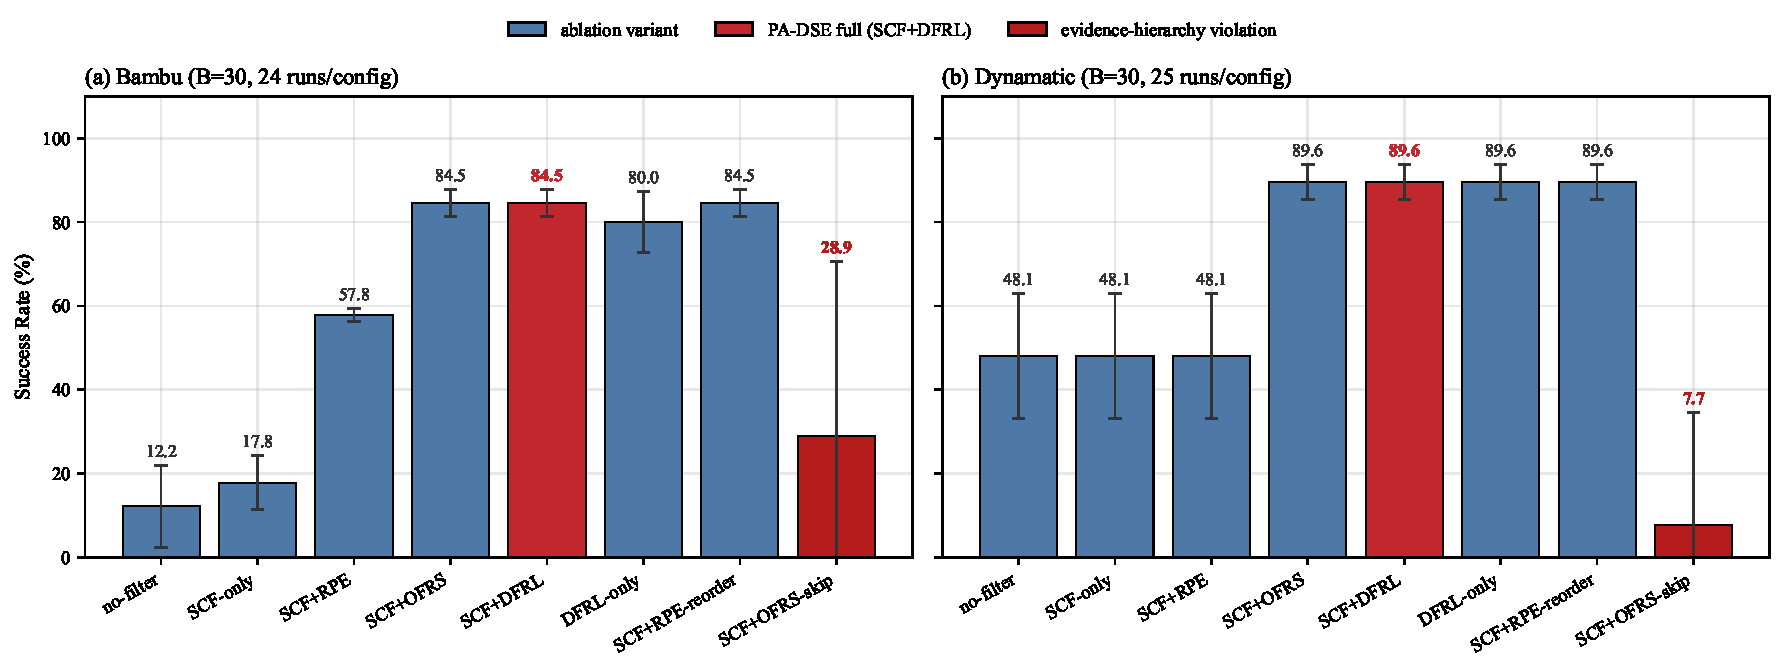
\includegraphics[width=\textwidth]{paper_figures/out/fig_ablation.pdf}
\caption{Ablation study visualization ($B{=}30$). PA-DSE full configuration (SCF+DFRL) highlighted in red. The rightmost bar (SCF+OFRS-skip, dark red) violates the evidence hierarchy by granting OFRS skip authority based on weak per-dimension evidence, producing order-of-magnitude larger variance and mean SR collapse on both tools.}
\label{fig:ablation}
\end{figure*}

\paragraph{OFRS is the dominant contributor to SR.} On Bambu, adding OFRS to SCF drives SR from $17.8\%$ (SCF-only) to $84.5\%$ (SCF+OFRS), a $+66.7$\,pp gain. On Dynamatic the effect is similar: $+41.5$\,pp from SCF-only ($48.1\%$) to SCF+OFRS ($89.6\%$). Across both tools, OFRS's online queue reordering is doing the heavy lifting at these budgets.

\paragraph{SCF provides a safety net on tools with static rules.} Comparing SCF+DFRL to DFRL-only isolates SCF's marginal value. On Bambu, SCF adds $+4.5$\,pp ($80.0\% \to 84.5\%$) by removing provably infeasible configurations before DFRL can be contaminated by their failures. On Dynamatic, SCF adds $0$\,pp because $\mathcal{C}_{\text{blk}} = \emptyset$. This asymmetry confirms the design stance: SCF's benefit is contingent on the tool exposing documented rules, but it is non-negative: it never hurts.

\paragraph{RPE is absorbed by OFRS under our budgets.} SCF+DFRL and SCF+OFRS are numerically identical ($84.5\%$ on Bambu, $89.6\%$ on Dynamatic). Yet SCF+RPE alone achieves only $57.8\%$ on Bambu, well below SCF+OFRS. Inspection of per-run logs reveals the mechanism: when OFRS is active, it reorders configurations matching heuristically-suppressed patterns to the tail of the queue. These are precisely the configurations RPE would have extracted signatures from. At $B{=}30$, OFRS's reordering means the budget is exhausted before the queue advances to where RPE would activate. The components are functional; they are not in use at this budget. Section~\ref{sec:b120} confirms this: at $B{=}120$, RPE activates and drives a $+36.3$\,pp SR gain over SCF+OFRS alone ($83.0\%$ vs.\ $46.7\%$, $p < 0.001$). Table~\ref{tab:theta_sensitivity} further shows that the RPE confidence threshold $\theta$ is a meaningful lever at this budget, with an $18.8$\,pp SR range across $\theta \in \{0.7, 0.8, 0.9\}$.

\paragraph{RPE-as-reorder degrades to SCF+OFRS.} Swapping RPE's action from \emph{skip} to \emph{reorder} yields identical results to SCF+OFRS ($84.5\%$ on Bambu). This is not a contradiction: when OFRS is already reordering by failure risk, adding RPE's risk-based reorder is redundant. The ablation confirms that RPE's distinct contribution is its \emph{skip} action, not any reordering signal.

\paragraph{Allowing OFRS to skip catastrophically increases variance.} The SCF+OFRS-as-skip configuration, which permits OFRS to hard-skip configurations at a risk threshold of $0.85$, produces mean SR $28.9\%$ with $\sigma{=}41.8$ on Bambu and $7.7\%$ with $\sigma{=}26.8$ on Dynamatic. These variances are an order of magnitude larger than any other configuration. On some runs OFRS's first-order marginal statistics happen to align with true failure causes and the run succeeds; on others, OFRS prunes feasible configurations based on noisy single-dimension correlations and the run collapses. This demonstrates that granting unstructured marginal statistics skip authority, without the consistency-and-contrast guards that RPE imposes (type-specific filtering, discriminative dimension selection, conservatively-smoothed confidence threshold), leads to catastrophic outcomes. The lesson is not merely that ``weak evidence should not drive strong actions'' in the abstract, but that the specific safeguards RPE provides are load-bearing.

\paragraph{Summary.} The ablation confirms three tenets of the evidence hierarchy: (i)~SCF's permanent block is safe only because it uses provable evidence; (ii)~OFRS's reordering is safe despite weak evidence because the action is weak (reorderable); (iii)~crossing these (allowing OFRS to skip) breaks the hierarchy and performance collapses.

% ------------------------------------------------------------
\subsection{Sensitivity to RPE Confidence Threshold $\theta$}
\label{sec:theta_sensitivity}

The RPE activation threshold $\theta$ (\S\ref{sec:rpe}) governs how much concentrated evidence is required before a failure signature triggers hard skip. A lower $\theta$ activates signatures earlier (more aggressive pruning); a higher $\theta$ requires more evidence (more conservative). To probe the sensitivity of PA-DSE to this hyperparameter we sweep $\theta \in \{0.7, 0.8, 0.9\}$ on Bambu, all $8$ benchmarks, $5$ queue permutations per cell ($n{=}40$ runs per $\theta$), with all other hyperparameters at their defaults (\S\ref{sec:protocol}).

\textbf{Budget choice.} The ablation in Section~\ref{sec:ablation} established that at $B{=}60$ on Bambu, RPE rarely activates within a single run because OFRS reordering surfaces feasible configurations before enough same-type failures accumulate to trigger signature extraction. A meaningful sensitivity analysis must therefore be conducted at a budget where RPE actively contributes. We use $B{=}120$, twice the default budget, where RPE activation is consistently observed. Note that SR at $B{=}120$ is lower than at $B{=}60$ (Table~\ref{tab:main_bambu}) because the denominator doubles: the queue now extends into higher-risk regions that OFRS defers at $B{=}60$. The absolute number of feasible designs found is substantially larger ($\sim 100$ vs.\ $\sim 55$), but the per-evaluation success \emph{rate} decreases because the marginal evaluations are riskier.

\begin{table}[t]
\centering
\caption{Sensitivity of PA-DSE to the RPE confidence threshold $\theta$ (Bambu, $B{=}120$, $n{=}40$ per cell: $8$ benchmarks $\times$ $5$ permutations). The default $\theta{=}0.8$ used throughout the paper is in bold. SR varies by $18.8$\,pp across the swept range. The $0.1$\,pp difference between this table's $\theta{=}0.8$ row ($83.1\%$) and Table~\ref{tab:b120}'s PA-DSE row ($83.0\%$) reflects the different sample sizes ($n{=}40$ vs.\ $n{=}80$).}
\label{tab:theta_sensitivity}
\begin{tabular}{lrrrr}
\toprule
$\theta$ & SR (\%) & Wasted & TTFF (s) & Sig.\ activated \\
\midrule
$0.7$ & $88.1 \pm 0.7$ & $7.6$ & $9.3$ & $1.0$ \\
$\mathbf{0.8}$ \textbf{(default)} & $\mathbf{83.1 \pm 0.6}$ & $\mathbf{11.4}$ & $\mathbf{9.3}$ & $\mathbf{1.0}$ \\
$0.9$ & $69.3 \pm 0.4$ & $24.8$ & $9.3$ & $1.0$ \\
\bottomrule
\end{tabular}
\end{table}

\textbf{Findings.} Table~\ref{tab:theta_sensitivity} summarises the sweep. Three observations are worth highlighting.
\begin{enumerate}
    \item \textbf{$\theta$ is a meaningful lever.} SR varies by $18.8$\,pp across the swept range ($88.1\%$ at $\theta{=}0.7$ down to $69.3\%$ at $\theta{=}0.9$), and Wasted varies by $3\times$ ($7.6 \to 24.8$). Variance within each $\theta$ cell is small ($\sigma \leq 0.7$\,pp), so the trend is statistically clean and not a sampling artifact.
    \item \textbf{Activation timing, not count, drives the trend.} Across all $120$ runs the number of activated signatures is consistently exactly $1$. The trend is therefore driven by \emph{when} the signature activates: at $\theta{=}0.7$, activation requires as few as $5$ same-type failures with zero counterexamples ($5/(5{+}0{+}2) \approx 0.71 \geq 0.7$), so the signature triggers early in the run and most of the remaining budget benefits from the hard skip. At $\theta{=}0.8$ the requirement rises to $8$ failures ($8/10 = 0.8$), and at $\theta{=}0.9$ to $18$ ($18/20 = 0.9$), which often occurs only near the end of the budget, yielding little benefit. This is the core mechanism the evidence-hierarchy formulation predicts.
    \item \textbf{Default $\theta{=}0.8$ is a balanced choice.} It sits midway between the aggressive $0.7$ and the conservative $0.9$ regimes, accepting some loss in SR relative to $0.7$ in exchange for tighter activation evidence ($\geq 8$ failures versus $5$ at $\theta{=}0.7$). For a deployment that prioritises raw throughput at large budgets, $\theta{=}0.7$ is preferable; for deployments where false skips are costly (e.g.\ when probe auditing is disabled), $\theta{=}0.9$ may be safer despite the SR cost.
\end{enumerate}

The sweep also serves as a cross-check on the budget-dependence claim of \S\ref{sec:ablation}: at $B{=}60$ the same sweep shows essentially no $\theta$ dependence (data not shown for brevity), because RPE rarely activates regardless of $\theta$. Sensitivity to $\theta$ is therefore conditional on RPE being in scope, which is itself conditional on budget being large enough for type-specific failure evidence to accumulate.

% ------------------------------------------------------------

\subsection{RPE Contribution at Extended Budget}
\label{sec:b120}

The ablation in Section~\ref{sec:ablation} showed that at $B{=}30$ and $B{=}60$, RPE does not activate because OFRS reordering exhausts the budget before sufficient type-specific failure evidence accumulates. To verify that RPE contributes at larger budgets, we run all methods at $B{=}120$ on Bambu (Table~\ref{tab:b120}), adding SCF+OFRS (PA-DSE without RPE) as an explicit ablation control.

\begin{table}[t]
\centering
\caption{Bambu at $B{=}120$ ($n{=}80$ runs per method: 8 benchmarks $\times$ 10 seeds/permutations). SCF+OFRS is PA-DSE with RPE disabled. The $+36.3$\,pp gap between PA-DSE and SCF+OFRS isolates RPE's contribution ($p < 0.001$, Wilcoxon). RF and SCF+OFRS exhibit $\sigma{=}0.0$ because at $B{=}120$ both methods have observed enough configurations to fully rank-order the active set, leaving no seed- or permutation-induced variation. PA-DSE's $\sigma{=}0.6$ reflects the residual stochasticity of probe auditing ($p_{\text{probe}}{=}0.05$).}
\label{tab:b120}
\begin{tabular}{lrrrr}
\toprule
Method & SR (\%) & Wasted & UQoR & Sigs \\
\midrule
Random          & 13.7 \std{2.1}  & 103.6 &  9.8 & -- \\
Filtered Random & 19.8 \std{1.4}  &  96.2 & 12.8 & -- \\
SA              &  7.2 \std{14.7} & 111.3 &  3.2 & -- \\
GA              & 31.8 \std{14.0} &  81.8 & 13.9 & -- \\
GP-BO           & 43.2 \std{0.5}  &  68.2 & 16.7 & -- \\
RF              & 46.7 \std{0.0}  &  64.0 & 19.1 & -- \\
SCF+OFRS        & 46.7 \std{0.0}  &  64.0 & 19.1 & 0 \\
\textbf{PA-DSE} & \textbf{83.0} \std{0.6} & \textbf{11.5} & \textbf{19.1} & \textbf{1.0} \\
\bottomrule
\end{tabular}
\end{table}

\begin{figure}[t]
\centering
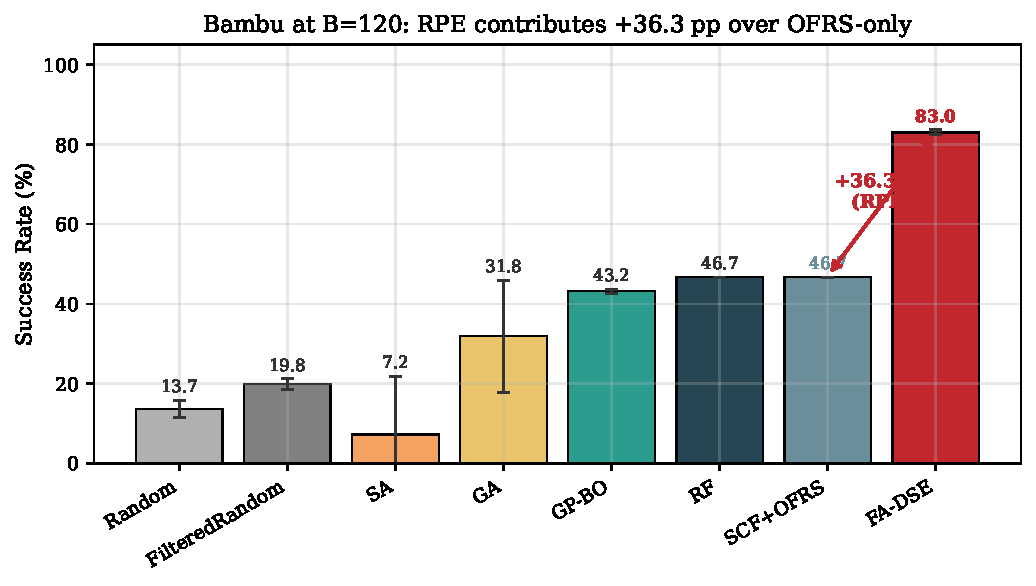
\includegraphics[width=\columnwidth]{paper_figures/out/fig_b120_bambu.pdf}
\caption{Bambu at $B{=}120$. RPE activates one signature per run, hard-skipping $\sim 213$ matching configurations and driving a $+36.3$\,pp SR gain over SCF+OFRS (which is identical to RF at this budget).}
\label{fig:b120}
\end{figure}

At $B{=}120$, RPE activates exactly one signature per run (the \texttt{pipeline\_phi\_conflict} pattern), which matches $\sim 213$ configurations in the $420$-point space; RPE hard-skips all such configurations remaining in the queue at activation time. This single signature drives PA-DSE from $46.7\%$ (identical to SCF+OFRS and RF) to $83.0\%$, a $+36.3$\,pp gain ($p < 0.001$, Wilcoxon signed-rank test over 80 paired runs). The mechanism behind this gain warrants explicit framing: because SR is the fraction of \emph{evaluated} configurations that synthesized successfully, RPE's hard-skipping shrinks the denominator. PA-DSE consumes approximately $68$ of the $120$ available calls and discovers $\sim 57$ feasible designs; SCF+OFRS consumes the full $120$ calls and discovers $\sim 56$. The two methods reach a comparable absolute count of feasible designs, but PA-DSE does so without spending the remaining $\sim 52$ calls on the pipeline-conflict region. The $+36.3$\,pp SR figure is therefore best read as a calls-to-success efficiency gain, not as a discovery gain---which is precisely the contribution attributed to RPE in the evidence hierarchy. Probe auditing consumes approximately $1.5\%$ of the budget actually consumed (an average of $1.0$ probe per run); probes fail in every run, confirming the signature's validity across the full benchmark suite.

The mechanism is clear: at $B{=}60$, OFRS surfaces feasible configurations fast enough that the budget is exhausted before $\tau{=}2$ same-type failures accumulate in the queue's reachable prefix. At $B{=}120$, the queue extends into the pipeline-conflict region, RPE observes repeated \texttt{pipeline\_phi\_conflict} failures, extracts a discriminative signature, and hard-skips matching configurations not yet evaluated ($\sim 213$ on average per run) for the remainder of the budget. OFRS alone cannot achieve this because its per-dimension marginal statistics do not distinguish pipeline conflicts from other failure types. This validates the evidence hierarchy: RPE's type-specific, concentrated evidence justifies the strong action (hard skip) that OFRS's mixed-type marginal statistics cannot.

\subsection{Overhead}
\label{sec:overhead}

Table~\ref{tab:overhead} reports the per-iteration algorithmic overhead of each PA-DSE layer, compared to the corresponding synthesis cost. On Bambu, total PA-DSE overhead is $5.3$\,ms per iteration, versus $\approx 2504$\,ms of synthesis: a ratio of $1:474$. On Dynamatic the ratio is $1:4000$, reflecting the higher synthesis cost of MILP-based buffer placement. By either measure, algorithmic overhead is negligible.

\begin{table*}[t]
\centering
\caption{Per-iteration overhead decomposition (ms). PA-DSE's algorithmic cost is $<0.22\%$ of synthesis cost on Bambu and $<0.04\%$ on Dynamatic.}
\label{tab:overhead}
\begin{tabular}{lrrrrr}
\toprule
Tool      & SCF  & RPE  & OFRS & Algo.\ total & Synthesis \\
\midrule
Bambu     & 0.086 & 0.169 & 5.030 & 5.285 & 2503.7 \\
Dynamatic & 0.029 & 0.069 & 1.934 & 2.032 & 8127.3 \\
\bottomrule
\end{tabular}
\end{table*}

\begin{figure}[t]
\centering
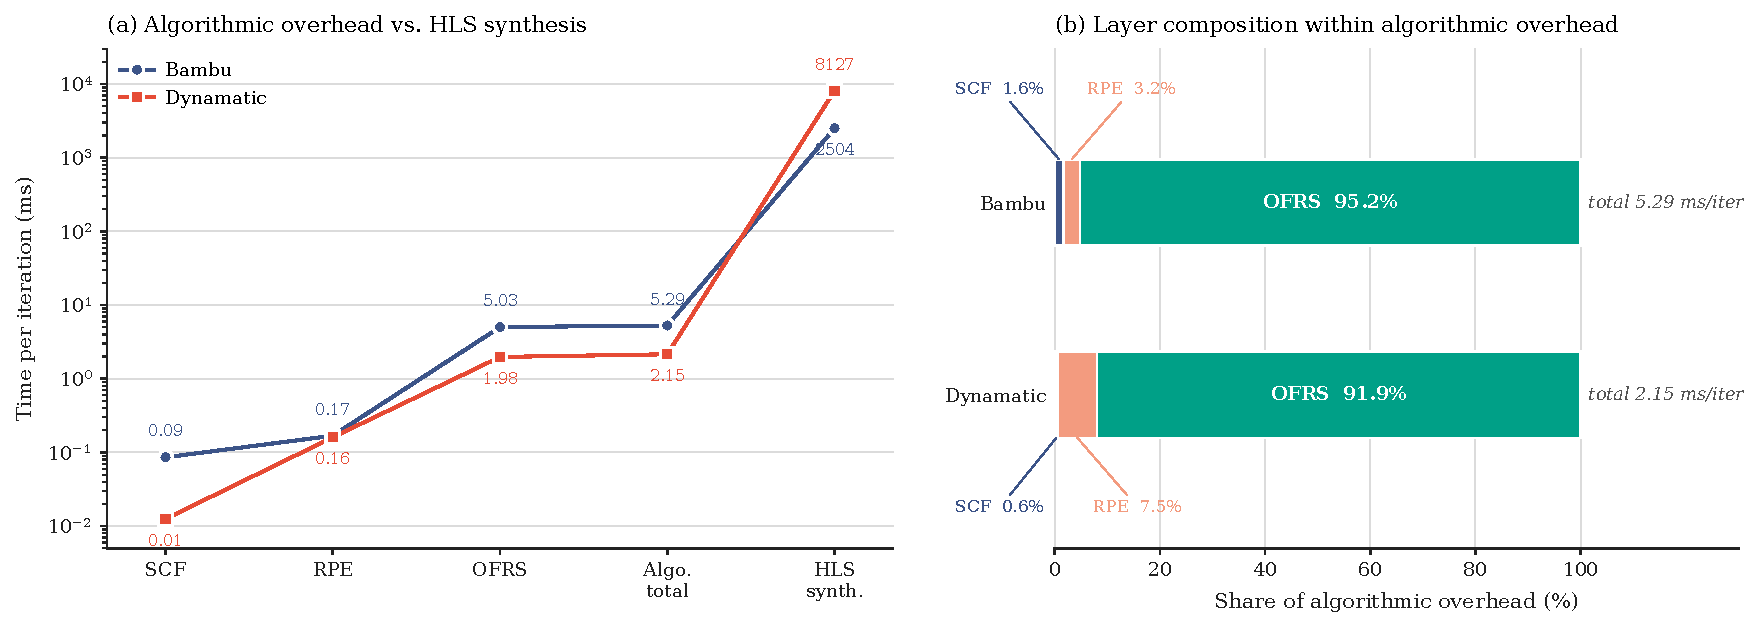
\includegraphics[width=\columnwidth]{paper_figures/out/fig_overhead.pdf}
\caption{Overhead analysis. (a) Per-iteration algorithmic cost is two-to-three orders of magnitude below synthesis cost on both tools. (b) Within the algorithmic overhead, OFRS dominates (it performs a queue sort each iteration); SCF and RPE are near-zero.}
\label{fig:overhead}
\end{figure}

OFRS dominates the algorithmic overhead ($95\%$ on Bambu, $92\%$ on Dynamatic) because it performs a full-queue sort every iteration. SCF is essentially free (rules fire once at initialization), and RPE's overhead is concentrated in a small number of signature-extraction calls per run. For design spaces substantially larger than ours, the OFRS sort could be replaced by an incremental priority queue with $O(\log n)$ update; we have not needed this optimization for the scales evaluated here.


\section{Discussion and Limitations}
\label{sec:discussion}

\subsection{When PA-DSE Helps, and When It Does Not}

PA-DSE is most effective in the regime our evaluation targets: small-to-moderate exploration budgets on design spaces where a non-trivial fraction of configurations are infeasible. Outside this regime its advantages diminish, and we state the limits explicitly.

\textbf{Very small budgets ($B < n_{\min}$).} OFRS requires $n_{\min}{=}5$ observations per dimension before its relevance weights stabilize. Below this threshold, OFRS falls back to a passive mode that preserves the SCF-established prior (active configurations first, suppressed last). In this regime PA-DSE behaves like Filtered Random with a mild heuristic ordering bias. At $B{=}10$ we would expect the gap to RF to narrow.

\textbf{Large budgets ($B \gg |\mathcal{C}_{\text{act}}|$).} At budgets approaching the full active-set size, every method converges to the same coverage. The pertinent question becomes not SR but QoR quality, where learned surrogates with offline training can leverage more data. PA-DSE is not designed for this regime.

\textbf{Tools without documented incompatibility rules.} On Dynamatic, SCF reduces to a no-op and PA-DSE's SR lead over the best baseline narrows to $+1.1$\,pp. The more distinctive advantage shifts to TTFF ($34.2$\,s vs.\ $67.0$\,s, nearly $2\times$ faster) and UQoR ($7.1$ vs.\ GP-BO $5.1$). DFRL alone is sufficient to match or exceed all baselines without tool-specific rule engineering. For tools whose failure distribution is driven by runtime-detected issues (e.g., timing closure, resource overflow), DFRL's online learning provides a viable fallback.

\subsection{Quality--Reliability Tradeoff}
\label{sec:tradeoff}

Among methods with SR $\geq 85\%$, PA-DSE leads on reliability-oriented metrics (SR, Wasted, TTFF) and remains competitive on QoR (Table~\ref{tab:main_dynamatic}). The only methods with lower best latency (Random, GA) achieve SR below $65\%$, making them unsuitable for production use. We examine this tradeoff below.

\begin{figure*}[t]
\centering
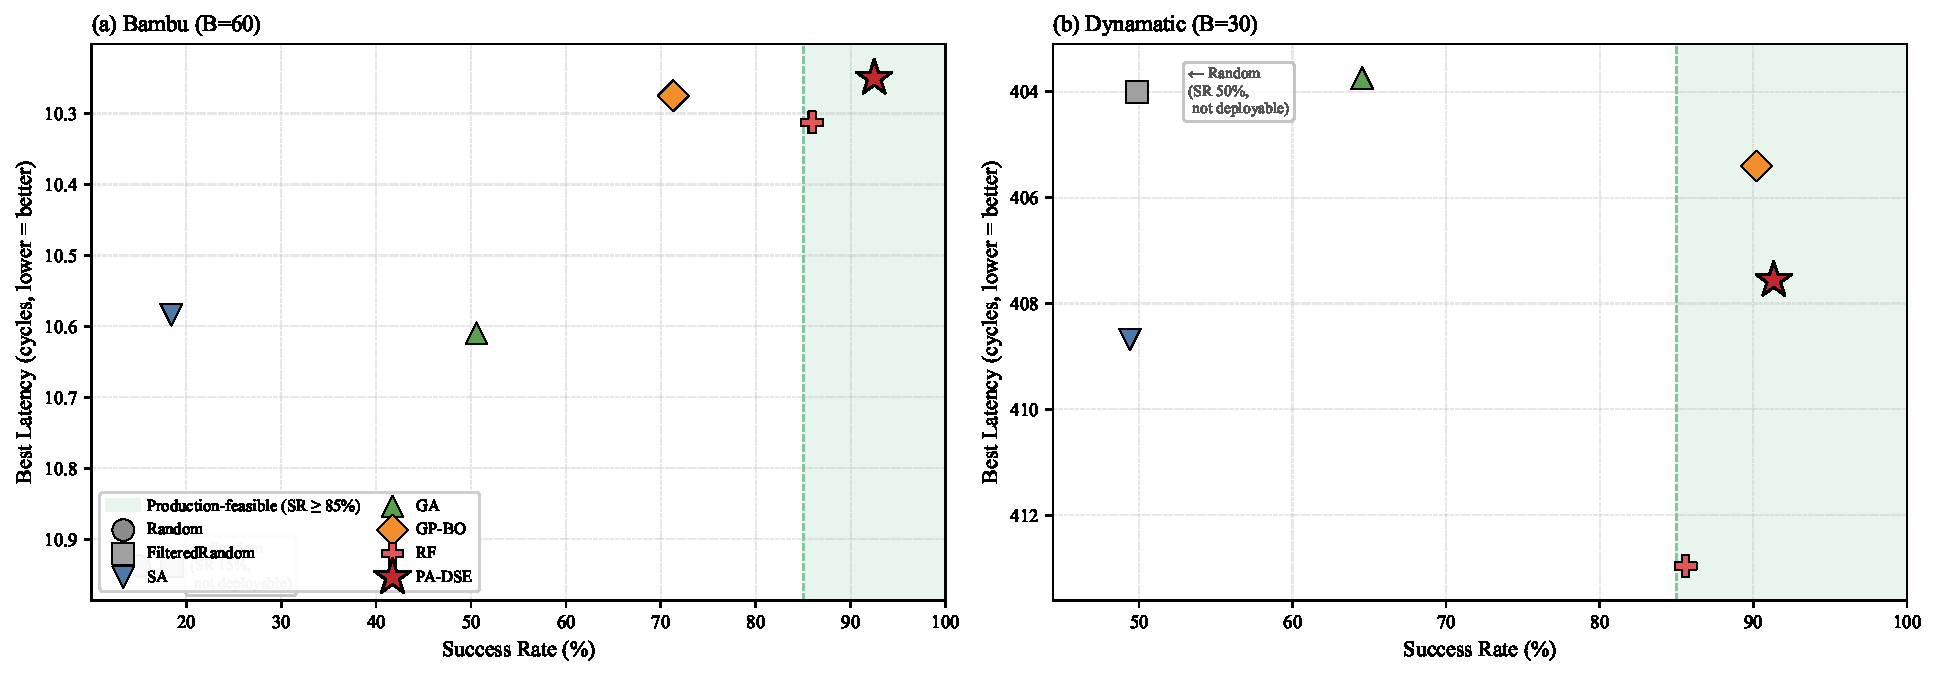
\includegraphics[width=\textwidth]{paper_figures/out/fig_pareto.pdf}
\caption{Reliability--quality Pareto trade-off: Success Rate (x-axis) vs.\ best latency (y-axis, lower is better). Shaded regions mark the production-feasible operating regime ($\text{SR} \geq 85\%$). On both Bambu (a) and Dynamatic (b), PA-DSE attains the Pareto frontier within the feasible region. On Dynamatic, methods outside the shaded region (Random, FilteredRandom, SA, GA) achieve lower best latency only by sacrificing tens of percentage points of SR, making them non-deployable as production policies regardless of their QoR numbers.}
\label{fig:pareto}
\end{figure*}

\textbf{The lat-strong baselines pay for it in SR.} Among the five non-trivial Dynamatic benchmarks, Random achieves lower best latency than PA-DSE but at catastrophic SR ($49.9\%$); GA shows a similar pattern ($64.5\%$ SR). These methods sample the design space broadly, which occasionally discovers low-latency configurations that PA-DSE does not reach within the limited budget, but the same broad sampling produces their catastrophic Wasted counts ($10$--$15$ calls per $30$-budget run). Figure~\ref{fig:pareto} visualizes this trade-off: methods inside the shaded production-feasible region ($\text{SR} \geq 85\%$) cluster around the Pareto frontier; methods outside trade tens of percentage points of SR for marginal latency gain. For a production DSE policy, a method that wastes one third to one half of every run on infeasible configurations is not deployable, regardless of its QoR numbers.

\textbf{Among deployable methods, PA-DSE compares favorably on user-visible cost.} GP-BO and RF are the only baselines with SR $\geq 85\%$. PA-DSE's SR is comparable to GP-BO ($91.3\%$ vs.\ $90.2\%$) while halving TTFF ($34.2$\,s vs.\ $67.0$\,s) and reducing Wasted ($2.6$ vs.\ $2.9$). UQoR is notably higher ($7.1$ vs.\ $5.1$). Best area is matched ($51.3$ vs.\ $51.3$). Best latency remains close to GP-BO ($407.6$ vs.\ $405.4$, a $2.2$-cycle / $0.5\%$ gap). Against RF, the gap is wider: SR $+5.7$\,pp, Wasted $-1.7$, TTFF $-32.8$\,s.



\textbf{Scope of comparison.} The meaningful comparison is among deployable methods (SR $\geq 85\%$), where PA-DSE compares favorably on reliability-oriented metrics while remaining close on QoR. Random and GA report lower best latency, but at SR below $65\%$, which limits their practical utility in production workflows. We adopt SR $\geq 85\%$ as a working deployment threshold: below this, more than one synthesis call in seven is wasted per run, which becomes a perceptible cost in interactive workflows where developers iterate tens of times a day. The qualitative conclusions are insensitive to the exact cutoff: at any threshold between $80\%$ and $90\%$, Random, Filtered Random, SA, and GA fall outside the deployable set, while PA-DSE, GP-BO, and RF fall inside.

\subsection{Decision Traceability}

A consequence of PA-DSE's design is that every skip decision is attributable to either (a)~a named static rule or (b)~a named RPE signature with a known support count and confidence. At the end of a run, one can inspect \texttt{signatures\_learned} and the associated \texttt{conditions} columns to see exactly which parameter combinations the algorithm treated as failure-prone. We call this \emph{decision traceability} rather than \emph{interpretability} to be precise: the framework exposes \emph{why the policy took an action}, but does not claim a causal explanation for the underlying tool's failure; a signature captures a statistical conjunction, not a root cause. This is still a pragmatic advantage over surrogate-based methods, where a confidently-predicted infeasibility is not attributable to a named piece of state at all.

\subsection{Generalization Across Runs}

PA-DSE's DFRL state does not persist across runs. Each invocation starts with empty RPE signatures and empty OFRS statistics, re-learning within the budget. This is a deliberate choice: failure signatures are strongly benchmark-dependent (e.g., a pipeline accumulation conflict appears only in kernels with accumulation loops), and persisting them across benchmarks risks false skips. Cross-run persistence for the \emph{same} benchmark is a natural extension: hashing the source AST and caching previously-learned signatures would yield a warm-start variant. We have not implemented this.

\subsection{Threats to Validity}

\textbf{Tool versions.} Our evaluation uses Bambu 0.9.8 and Dynamatic 2.0 with Gurobi 12.0. Different tool versions may expose different failure modes; the RPE signatures learned for Bambu 0.9.8 are not guaranteed to transfer to future releases.

\textbf{Benchmark suite.} Our eight benchmarks (shared across both tools) are small-to-medium in size ($< 1000$ lines of C each). For kernel-style benchmarks this is representative; for full-application HLS, longer compile times would shift the overhead ratio further in PA-DSE's favor, but the feasibility landscape may differ qualitatively.

\textbf{Permutation-based repetition.} For PA-DSE we report 10 queue permutations rather than 10 seeds. The two are mechanically equivalent for a deterministic algorithm (permutation fixes the initial queue order, a seed fixes internal randomness in a stochastic algorithm), but readers should note this is not a statistical sample of PA-DSE's stochasticity per se; PA-DSE is deterministic conditional on the queue order. The $p_{\text{probe}}{=}0.05$ introduces residual stochasticity at extended budgets where RPE activates (cf.\ Table~\ref{tab:b120}, $\sigma{=}0.6$ at $B{=}120$); at $B{=}60$ on Bambu, RPE does not activate and no probes are triggered, so the observed $\sigma{=}1.1$ reflects across-permutation variation alone.

\textbf{RF baseline fidelity.} Our RF baseline is a simplified online proxy for the AutoScaleDSE family; a faithful re-implementation would require offline corpus training across multiple HLS designs and tool versions. The RF numbers in this paper should be read as representative of what an online random-forest classifier achieves under our conditions, not as an upper bound on the learned-surrogate family.

\textbf{No direct comparison against recent surrogate methods.} We did not retrain recent GNN-based feasibility predictors (e.g., HGBO-DSE~\cite{kuang2023hgbo}, IronMan~\cite{wu2021ironman}) on our configuration spaces, as doing so would require retraining on our specific tool versions and pragma ranges. The RF baseline serves as a proxy for the learned-classifier family under our evaluation conditions. A direct comparison with offline-trained GNN surrogates would further contextualize PA-DSE's relative strengths and is planned as future work.


\section{Conclusion}
\label{sec:conclusion}

We presented PA-DSE, a feasibility-aware HLS design space exploration policy built around the principle that action strength must not exceed evidence strength. The policy has two layers: a static constraint filter (SCF) that permanently removes configurations matching tool-documented incompatibility rules, and a dynamic failure risk learner (DFRL) that accumulates evidence during a single exploration run and reorders the queue accordingly. DFRL has two sub-components, recurrent pattern extraction (RPE) for signature-based hard skipping and online failure risk scoring (OFRS) for continuous queue reordering, each restricted to actions its evidence can justify.

On eight Bambu benchmarks at $B{=}60$, PA-DSE achieves $92.5\%$ success rate with the lowest variance of any non-trivial method, outperforming a random-forest baseline by $+6.6$\,pp and reducing wasted synthesis calls by $\mathbf{1.9\times}$. On the same eight benchmarks evaluated on Dynamatic at $B{=}30$ (a tool with no applicable static rules, where SCF reduces to a no-op), PA-DSE reaches $91.3\%$ success rate on the five benchmarks with non-trivial failure rates and halves the time-to-first-feasible compared to the strongest baselines, with QoR closely matching deployable baselines (matched best area, full Pareto-vertex coverage, and best latency within $0.5\%$ of GP-BO). Three benchmarks achieve $100\%$ feasibility on Dynamatic but not on Bambu, a structural asymmetry that validates the two-layer design: SCF handles pragma-driven failures, DFRL handles graph-complexity-driven failures. An 8-way ablation confirms that each component is engaged in the way its evidence hierarchy position predicts: at the interactive budgets of our main evaluation ($B{=}30$--$60$), OFRS's weak-evidence online reordering is the dominant within-budget contributor, while RPE remains dormant because OFRS exhausts the budget before sufficient type-specific failure evidence accumulates; only at the extended budget $B{=}120$ does RPE activate and add $+36.3$\,pp over OFRS-only by hard-skipping configurations matching a learned pipeline-conflict signature. SCF's strong-evidence permanent block is a safety net on tools that expose one, and allowing OFRS to hard-skip (breaking the hierarchy) causes variance to explode by an order of magnitude. A sensitivity sweep of the RPE confidence threshold $\theta$ at $B{=}120$ confirms that activation timing, not signature count, drives performance, and that the default $\theta{=}0.8$ provides a balanced operating point between aggressive early activation ($\theta{=}0.7$, SR $88\%$) and conservative late activation ($\theta{=}0.9$, SR $69\%$). The total algorithmic overhead is $5.3$\,ms per iteration on Bambu and $2.0$\,ms on Dynamatic, negligible compared to the $2.5$\,s and $8.1$\,s per-call synthesis costs.

The framework requires no offline training and operates within a single exploration run; every skip decision is attributable to a named rule or signature with a known support count. We do not claim causal explanation of the tool's underlying behaviour. We view the principal contribution as a design pattern: strictly couple action strength to evidence strength, rather than a specific set of rules or scoring functions. Extensions we consider promising include QoR-aware queue reordering (e.g., novelty bonuses or density penalties) for scenarios where the success cloud is narrow, cross-run signature caching for repeated benchmark exploration, higher-order interaction-aware risk scoring for spaces where single-dimension statistics saturate, and integration with a probe-rate controller that actively modulates the quality--reliability tradeoff.

Code, raw experimental data, and a reproduction script for every table and figure in this paper are released at \url{https://github.com/jane09250410/hls-dse}.

% --------------------------------------------------------
% References
% --------------------------------------------------------
\bibliographystyle{IEEEtran}
{\small
\enlargethispage{4\baselineskip}
\bibliography{references}
}

\end{document}
